% Rapport du projet : calibration du modèle de Heston par réseau de neurones.
% Compilation : voir rapport/README.md (latexmk -pdf main.tex, ou LaTeX Workshop dans VS Code).
% Chaque section est dans son propre fichier (sections/), pour pouvoir écrire à plusieurs sans conflit Git.
% Les figures sont prises directement dans results/figures/ : relancer un notebook met le rapport à jour.

\documentclass[11pt,a4paper]{article}

\usepackage[T1]{fontenc}
\usepackage[utf8]{inputenc}
\usepackage{lmodern}
\usepackage[french]{babel}
\usepackage[margin=2.5cm]{geometry}
\usepackage{microtype}
\usepackage{amsmath,amssymb}
\usepackage{graphicx}
\graphicspath{{../results/figures/}{figures/}}
\usepackage{booktabs}
\usepackage[locale=FR]{siunitx}
\usepackage{caption}
\usepackage{subcaption}
\usepackage{float}
\usepackage{xcolor}
\usepackage[authoryear,round]{natbib}
\usepackage[hidelinks]{hyperref}
\usepackage[french,nameinlink]{cleveref}

% Les étiquettes utilisent « - » et pas « : » (babel french rend « : » actif, ce qui casse \cref).
% Notations
\newcommand{\pb}{\,\text{pb}}                     % point de base de volatilité (0,01 point de vol)
\newcommand{\ie}{c'est-à-dire}
\newcommand{\afaire}[1]{\textcolor{red}{\textbf{[À faire : #1]}}}   % à supprimer dans la version finale

\title{Calibration du modèle de Heston par réseau de neurones}
\author{Adam Boufous \and Elise Ricourt \and Matthieu Galtier \and Omar Guenoun}
\date{Projet de Deep Learning --- Université Paris Dauphine-PSL --- novembre 2026}

\begin{document}

\maketitle

\begin{abstract}
Calibrer le modèle de Heston demande des centaines d'évaluations de la surface de volatilité, chacune calculée par
une méthode de Fourier. Comme \citet{horvath2021}, nous entraînons un réseau de neurones à prédire la surface à
partir des cinq paramètres, sur \num{50000} surfaces simulées, puis nous l'utilisons à la place de Fourier pour
calibrer. Après le choix de l'architecture ($2\times128$) et de l'entraînement (Adam, He, GELU), le réseau fait
\num{2.67}\pb\ d'erreur moyenne sur le test et répond plus de 70 fois plus vite que Fourier. Il est plus précis que
les méthodes d'apprentissage classiques dès qu'il apprend sur toutes les données. En calibration, il retrouve les
paramètres de surfaces simulées et donne sur le SPX les mêmes résultats que Fourier, des centaines de fois plus
vite ; son coût d'entraînement est amorti en quelques calibrations.
\end{abstract}

\tableofcontents

\section{Introduction}
\label{sec-introduction}

Calibrer un modèle, c'est choisir ses paramètres pour que les prix qu'il donne collent aux prix du marché. Pour le
modèle de \citet{heston1993}, il n'existe pas de formule fermée des prix : chaque surface de volatilité implicite
se calcule par une méthode de Fourier, qui prend quelques millisecondes. Un optimiseur demande des centaines
d'évaluations de la surface, et une banque recalibre ses modèles plusieurs fois par jour, sur de nombreux sous-jacents :
le pricer devient le goulot d'étranglement.

\citet{horvath2021} proposent de séparer le travail en deux temps. Hors ligne, un réseau de neurones apprend la
fonction qui associe aux paramètres du modèle la surface de volatilité sur une grille fixe de maturités et de
strikes ; les exemples d'entraînement sont produits une fois pour toutes avec le pricer exact. En ligne, la
calibration utilise le réseau à la place du pricer : une évaluation n'est plus qu'un passage avant dans un petit
réseau, beaucoup plus rapide. Le coût est déplacé vers la génération des données et l'entraînement, qui ne sont
faits qu'une fois.

Nous appliquons cette méthode au modèle de Heston et cherchons à répondre à quatre questions :
\begin{itemize}
  \item quelle architecture choisir, sachant que le réseau doit être à la fois précis et au moins dix fois plus
  rapide que le pricer Fourier ;
  \item comment l'entraîner (optimiseur, initialisation, fonction d'activation) ;
  \item un réseau de neurones fait-il mieux que des méthodes d'apprentissage classiques sur ce problème ;
  \item la calibration par le réseau est-elle aussi bonne que la calibration par Fourier, sur des surfaces
  simulées et sur le marché (SPX), et à partir de combien de calibrations le temps d'entraînement est-il
  rentabilisé.
\end{itemize}

La \cref{sec-donnees} présente le modèle, le pricer de référence, le jeu d'entraînement et les surfaces de marché.
La \cref{sec-mise-en-oeuvre} décrit l'organisation du code. Les \cref{sec-architectures,sec-entrainement}
choisissent l'architecture puis l'entraînement du réseau. La \cref{sec-dl-vs-ml} le compare à des méthodes
classiques, et la \cref{sec-calibration} l'utilise pour calibrer. La \cref{sec-conclusion} conclut.

% Étape 0 : données.
% Sources : julia/, configs/base.yaml, notebooks/00_donnees.ipynb, results/etape0/, data/spx/.

\section{Données}
\label{sec-donnees}

Le réseau apprend la fonction qui associe aux cinq paramètres de Heston une surface de volatilité implicite.
Il faut donc un pricer de référence fiable, un jeu de surfaces simulées qui couvre le domaine utile, et des
surfaces de marché pour l'étape de calibration (\cref{sec-calibration}). Cette section les décrit et explique nos
choix.

\subsection{Le modèle et la grille}
\label{sec-modele}

On écrit le modèle de \citet{heston1993} directement sur le prix forward $F_t$ (taux nul, dividendes inclus dans
le forward), avec une variance instantanée $v_t$ qui revient vers sa moyenne :
\begin{equation}
  \frac{dF_t}{F_t} = \sqrt{v_t}\, dW_t, \qquad
  dv_t = \kappa(\theta - v_t)\, dt + \xi \sqrt{v_t}\, dZ_t, \qquad
  d\langle W, Z\rangle_t = \rho\, dt .
  \label{eq-heston}
\end{equation}
Les cinq paramètres sont la variance initiale $v_0$, la variance de long terme $\theta$, la vitesse de retour
$\kappa$, la volatilité de la variance $\xi$ et la corrélation $\rho$. Le ratio de \citet{feller1951}
$2\kappa\theta/\xi^2$ indique si la variance peut toucher zéro (ratio inférieur à 1) ; on y reviendra.

On normalise $F_0 = 1$ : le strike $K$ est alors directement la moneyness $K/F_0$. Une surface est l'ensemble des
volatilités implicites de Black-76 \citep{black1976} sur une grille fixe de
\num{8} maturités ($T \in \{0{,}1 ; 0{,}3 ; 0{,}6 ; 0{,}9 ; 1{,}2 ; 1{,}5 ; 1{,}8 ; 2\}$ ans) et
\num{11} strikes ($K$ de \num{0.5} à \num{1.5} par pas de \num{0.1}), soit \num{88} valeurs : c'est la sortie
du réseau. Les erreurs sont exprimées en points de base de volatilité ($1\pb = \num{0.01}$ point de vol,
par exemple \SI{20.00}{\percent} au lieu de \SI{20.01}{\percent}).

\subsection{Le pricer de référence}
\label{sec-pricer}

Le pricer est écrit en Julia (\texttt{julia/src/HestonFourier.jl}) pour la vitesse. Pour une maturité donnée, il
calcule les prix de toutes les options de la grille par la méthode COS de \citet{fang2008} : la densité du
log-rendement $x = \log(F_T/F_0)$ est développée en série de cosinus sur un intervalle $[a,b]$,
\begin{equation}
  f(x) \approx {\sum_{k=0}^{N-1}}' A_k \cos\!\Big(k\pi\frac{x-a}{b-a}\Big), \qquad
  A_k = \frac{2}{b-a}\, \mathrm{Re}\Big[\varphi\Big(\frac{k\pi}{b-a}\Big) e^{-ik\pi a/(b-a)}\Big],
\end{equation}
où $\varphi$ est la fonction caractéristique de Heston, écrite sous la forme « little Heston trap » de
\citet{albrecher2007} pour éviter les discontinuités du logarithme complexe. Les coefficients $A_k$ sont calculés
une seule fois par maturité ; chaque strike ne coûte ensuite qu'une somme. On price toujours l'option hors de la
monnaie (put si $K<1$, call sinon) : son prix est petit mais calculé directement, sans passer par la parité
call-put qui ferait perdre de la précision. Le nombre de termes part de $N = 256$ et double tant que
$|\varphi(N\pi/(b-a))| > 10^{-15}$. La volatilité implicite est obtenue en inversant la formule de Black-76 par la
méthode de Brent.

\paragraph{Trois corrections de précision.} En vérifiant le pricer contre une méthode indépendante (formule de
\citet{lewis2000}, intégration numérique), nous avons trouvé et corrigé trois défauts :
\begin{itemize}
  \item l'intervalle $[a,b]$ est centré sur la moyenne $c_1$ du log-rendement, avec une largeur proportionnelle à
  son écart-type $\sqrt{c_2}$. La formule fermée de $c_2$ que nous utilisions donnait une variance
  \emph{négative} pour environ \SI{20}{\percent} des paramètres tirés. Nous calculons désormais $c_1$ et $c_2$
  directement à partir de la fonction caractéristique ($\log\varphi(u) \approx i c_1 u - c_2 u^2/2$, par
  différences finies) ;
  \item un intervalle de $\pm 12$ écarts-types est trop étroit quand la condition de Feller est très violée : la
  queue gauche de la densité est alors épaisse, et l'erreur pouvait atteindre plusieurs centaines de points de
  base. Nous prenons $\pm 32$ écarts-types, avec une borne droite plafonnée à $b = 10$ (au-delà, le terme $e^{b}$
  du calcul des calls fait perdre de la précision, alors qu'un rendement de $e^{10}$ n'a aucune probabilité) ;
  \item en dessous d'un prix de $10^{-10}$, l'erreur numérique de la méthode (quelques $10^{-12}$) fausse la
  volatilité implicite de plusieurs points de base : ces points sont marqués comme manquants (NaN), au lieu du
  seuil de $10^{-12}$ utilisé au départ.
\end{itemize}
Après correction, l'écart maximal avec la formule de Lewis est de \SI{0.002}{\pb} sur près de \num{39000} points,
choisis au hasard et parmi les cas les plus difficiles (forte volatilité, maturité longue, condition de Feller très
violée). Le pricer est couvert par \num{274} tests automatiques : prix de référence publié par \citet{fang2008},
limite de Black-Scholes, absence d'arbitrage (prix des calls décroissants et convexes en $K$), et les cas
difficiles ci-dessus.

\paragraph{Une copie en Python.} Le même pricer existe en Python (module \texttt{heston\_cos}), pour vérifier
le code Julia et pouvoir calibrer sans Julia. Recalculées en Python à partir des mêmes paramètres,
les \num{50000} surfaces d'entraînement sont identiques : les NaN sont exactement aux mêmes endroits, et l'écart
est de \SI{1e-6}{\pb} en moyenne (\SI{0.07}{\pb} au maximum, sur des calls très loin de la monnaie dont le prix est
proche du seuil).

\subsection{Le domaine des paramètres}
\label{sec-plages}

Le réseau n'apprend que ce qu'on lui montre : le domaine de tirage des paramètres doit couvrir les surfaces qu'on
voudra calibrer, sans gaspiller des exemples sur des régimes irréalistes. Le \cref{tab-plages} donne notre choix
(\texttt{configs/base.yaml}).

\begin{table}[H]
  \centering
  \caption{Domaine de tirage des paramètres, comparé au code Heston de \citet{horvath2021}.}
  \label{tab-plages}
  \small
  \begin{tabular}{lccl}
    \toprule
    Paramètre & Notre domaine & \citet{horvath2021} & Commentaire \\
    \midrule
    $v_0$      & $[0{,}0049 ; 0{,}16]$ & $[0{,}0001 ; 0{,}04]$ & vol initiale de \SI{7}{\percent} à \SI{40}{\percent} \\
    $\theta$   & $[0{,}01 ; 0{,}16]$   & $[0{,}01 ; 0{,}20]$   & vol de long terme de \SI{10}{\percent} à \SI{40}{\percent} \\
    $\kappa$   & $[0{,}5 ; 10]$        & $[1 ; 10]$            & \\
    $\xi$      & $[0{,}1 ; 1{,}5]$     & $[0{,}01 ; 1]$        & souvent supérieur à 1 sur le SPX \\
    $\rho$     & $[-0{,}95 ; -0{,}1]$  & $[-0{,}95 ; -0{,}1]$  & toujours nettement négatif sur le SPX \\
    Feller     & $2\kappa\theta/\xi^2 \geq 0{,}1$ & $\geq 1$ pour tout leur jeu & \\
    \bottomrule
  \end{tabular}
\end{table}

L'article de \citet{horvath2021} ne donne pas de domaine pour Heston ; les valeurs du tableau viennent de leur code
public \citep{horvathcode}. Nous ne les avons pas reprises : avec $v_0$ descendant à $10^{-4}$ (une volatilité de
\SI{1}{\percent}), plus des trois quarts des surfaces contiendraient des points non calculables avec notre pricer, et
$\xi \leq 1$ est trop étroit pour le SPX (\cref{sec-spx}).

\paragraph{Tirer la volatilité, pas la variance.} Un tirage uniforme de $v_0$ et $\theta$ concentre les exemples
sur les fortes volatilités, puisque la volatilité est la racine de la variance. Avec notre premier domaine
($v_0, \theta \in [0{,}01 ; 0{,}25]$, tirés uniformément), la volatilité à la monnaie à 1 mois avait une médiane de
\SI{36}{\percent}, \SI{70}{\percent} des surfaces dépassaient \SI{30}{\percent}, et seulement \SI{17}{\percent}
tombaient entre \SI{10}{\percent} et \SI{25}{\percent}, la zone habituelle du SPX. Nous tirons donc
$\sqrt{v_0}$ et $\sqrt{\theta}$ uniformément : la médiane passe à \SI{24}{\percent}, et \SI{52}{\percent} des
surfaces sont dans la zone \SIrange{10}{25}{\percent} (\cref{fig-vols-atm}).

\paragraph{Feller.} Nous n'imposons pas la condition de Feller (ratio $\geq 1$) : les calibrations de marché la
violent souvent, et près de la moitié de nos surfaces (\SI{49}{\percent}) la violent. Nous excluons seulement les violations
extrêmes (ratio $< 0{,}1$, soit \SI{7}{\percent} des tirages), où la densité est si asymétrique que même le pricer
corrigé perd en précision, et qui sont loin des calibrations du SPX (ratio de \num{0.17} à \num{0.19},
\cref{tab-spx-calibration}).

\begin{figure}[H]
  \centering
  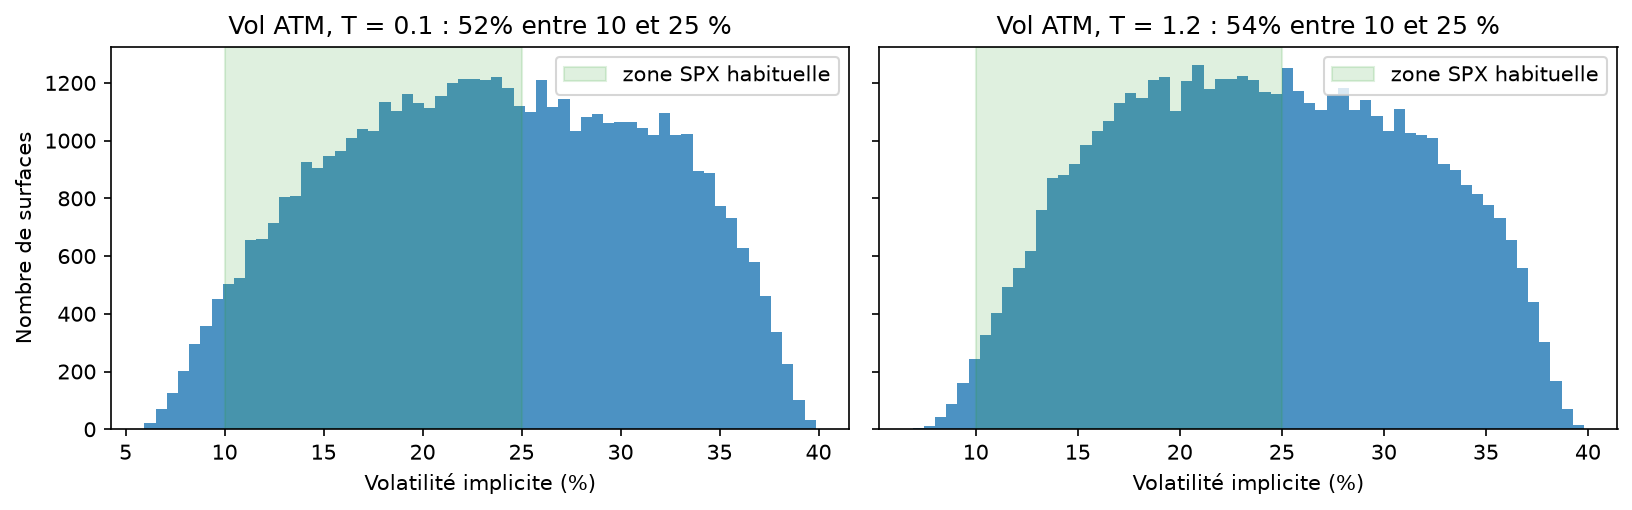
\includegraphics[width=\textwidth]{etape0_vols_atm}
  \caption{Répartition de la volatilité implicite à la monnaie ($K=1$) dans le jeu d'entraînement, à 1 mois et à
  1,2 an. La bande verte est la zone habituelle du SPX.}
  \label{fig-vols-atm}
\end{figure}

\subsection{Le jeu d'entraînement}
\label{sec-jeu}

Nous avons généré \num{50000} surfaces (\texttt{julia/generate\_data.jl}, graine \num{42}), découpées en
\num{40000} pour l'entraînement, \num{5000} pour la validation et \num{5000} pour le test (\SI{80}{\percent} /
\SI{10}{\percent} / \SI{10}{\percent}). Les paramètres sont tirés avant le calcul parallèle : le fichier est
identique quel que soit le nombre de threads. La \cref{fig-surfaces} montre quatre surfaces tirées au hasard : on
retrouve le skew négatif ($\rho<0$), qui s'aplatit quand la maturité augmente.

\begin{figure}[H]
  \centering
  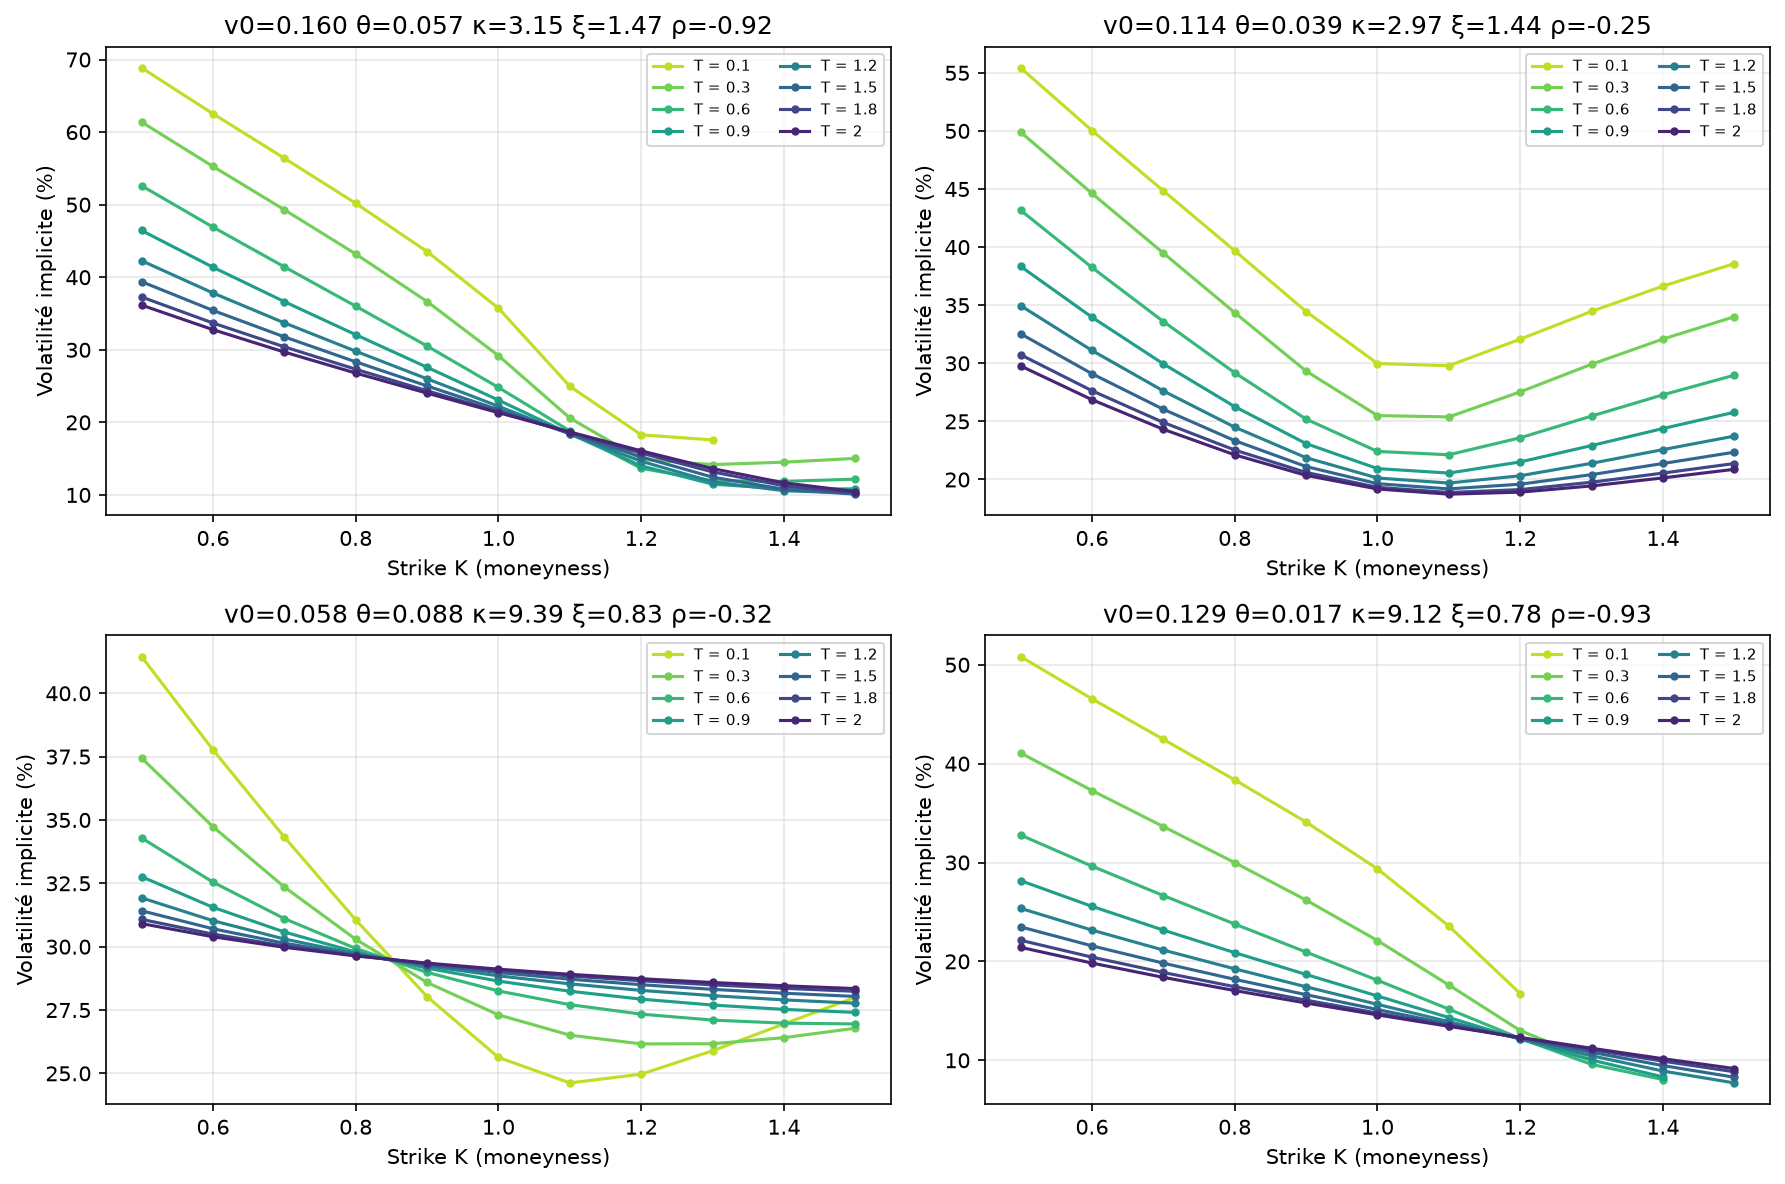
\includegraphics[width=\textwidth]{etape0_surfaces}
  \caption{Quatre surfaces du jeu d'entraînement, une courbe par maturité.}
  \label{fig-surfaces}
\end{figure}

\paragraph{Les points manquants.} Une option dont le prix est inférieur à $10^{-10}$ n'a pas de volatilité implicite
fiable : le point est marqué NaN. \SI{56.2}{\percent} des surfaces ont au moins un point manquant, mais cela ne
représente que \SI{1.9}{\percent} des points (\num{83827} sur \num{4400000}). Ils sont presque tous à la maturité
d'un mois, sur les strikes extrêmes (\cref{fig-nan}) : \SI{34}{\percent} des surfaces à $K=0{,}5$, \SI{44}{\percent}
à $K=1{,}5$. Au-delà d'un mois, il ne reste que \SI{0.34}{\percent} de points manquants. Ces options ne sont de
toute façon pas cotées sur le marché. Nous gardons ces surfaces : la perte du réseau et les métriques ignorent
simplement les points manquants. Jeter les surfaces entières ferait perdre plus de la moitié du jeu.

\begin{figure}[H]
  \centering
  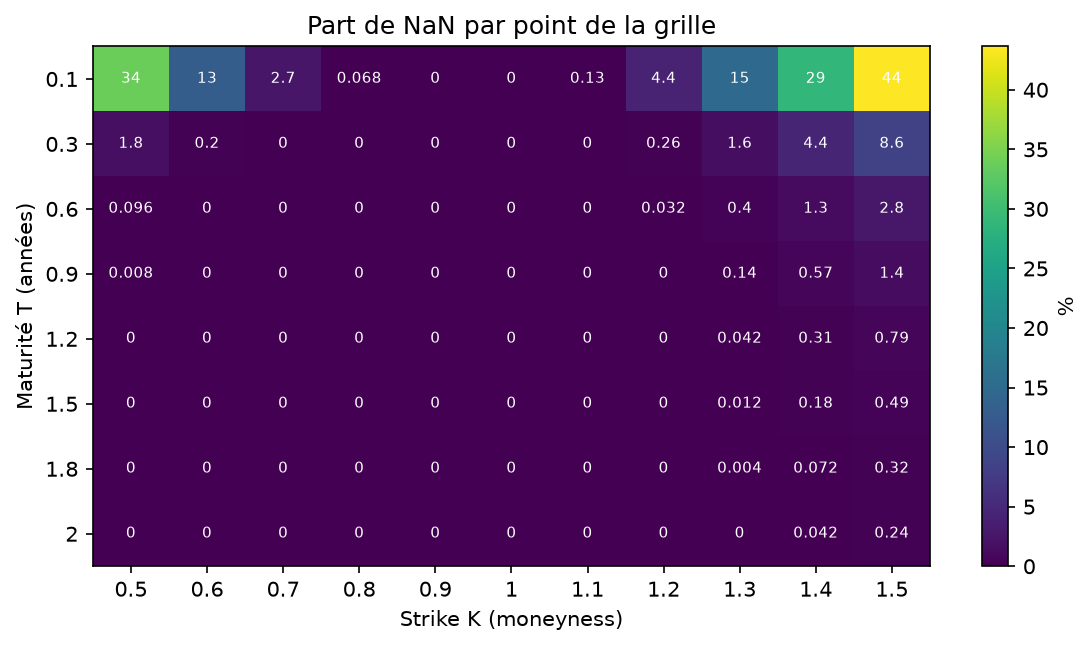
\includegraphics[width=0.85\textwidth]{etape0_nan}
  \caption{Part des surfaces où le point est manquant (NaN), en \%, pour chaque point de la grille.}
  \label{fig-nan}
\end{figure}

\subsection{Le coût de Fourier}
\label{sec-cout}

Le temps de référence que le réseau devra battre est celui d'une surface sur un seul cœur, inversion de
Black-76 comprise. Julia et Python sont mesurés de la même façon, sur les mêmes 200 jeux de paramètres (les 200
premières surfaces du jeu) : pour chaque jeu, un appel à blanc puis cinq mesures dont on garde la médiane ; le
temps retenu est la médiane sur les 200 jeux. Le \cref{tab-temps} compare les deux : Julia est cinq fois plus
rapide sur une surface et presque quatre fois plus rapide sur la génération complète, ce qui justifie de l'avoir
choisi pour la génération des données. Le temps d'une surface dépend beaucoup des paramètres (de \SI{0.9}{\ms} à
\SI{25}{\ms} en Julia), car le nombre de termes de la série COS nécessaire varie, d'où le choix de la médiane.

Ces mesures sont sensibles à la charge de la machine : mesurés pendant que d'autres calculs tournaient, les mêmes
codes prenaient deux à trois fois plus de temps. Tous les temps du projet sont donc mesurés machine au repos, sur
la même machine.

\begin{table}[H]
  \centering
  \caption{Temps de calcul (processeur AMD Zen 5, 20 threads).}
  \label{tab-temps}
  \begin{tabular}{lrrr}
    \toprule
    & Julia & Python & Python / Julia \\
    \midrule
    Une surface, un cœur (médiane)                   & \SI{2.29}{\ms}  & \SI{11.0}{\ms} & \num{4.8} \\
    Génération des \num{50000} surfaces (20 threads) & \SI{23.9}{\s}   & \SI{89.1}{\s}  & \num{3.7} \\
    \bottomrule
  \end{tabular}
\end{table}

Le pricer est réglé pour la précision plutôt que pour la vitesse. Un intervalle de troncature adapté au ratio de
Feller le rendrait environ \SI{30}{\percent} plus rapide, sans changer l'ordre de grandeur du gain du réseau.

\subsection{Les surfaces de marché (SPX)}
\label{sec-spx}

Pour l'étape de calibration, nous avons construit des surfaces réelles à partir des options sur l'indice S\&P 500
(SPX), des options européennes. Les cotations viennent de Yahoo Finance, téléchargées avec la bibliothèque
\texttt{yfinance} pendant les heures d'ouverture américaines. Le traitement (\texttt{src/heston\_nn/data/market.py})
suit les étapes suivantes :
\begin{enumerate}
  \item Nettoyage. On garde les échéances de 7 jours à 2,6 ans et les cotations dont le prix moyen
  (milieu de la fourchette achat-vente) dépasse \num{0.05} et dont la fourchette relative est inférieure à
  \SI{50}{\percent}.
  \item Forward et actualisation. La parité call-put $C - P = D\,(F - K)$ est une droite en $K$. Estimé
  échéance par échéance, le facteur d'actualisation $D$ est très bruité : le 20 novembre, les taux implicites
  allaient de \SI{-36}{\percent} à \SI{235}{\percent}, et une échéance mal estimée décalait toute une ligne de la
  surface d'environ un point de volatilité. Nous estimons donc \emph{un seul taux par jour} (médiane des échéances
  d'au moins trois mois), en déduisons $D = e^{-rT}$ pour toutes les échéances, puis le forward de chacune par
  $F = K + (C-P)/D$ sur les strikes proches de la monnaie.
  \item Volatilités implicites des options hors de la monnaie, par la formule de Black-76.
  \item Lissage. Pour chaque échéance, un smile SVI \citep{gatheral2014} est ajusté sur les strikes
  $K/F \in [0{,}4 ; 1{,}7]$.
  \item Projection sur la grille, par interpolation linéaire de la variance totale $\sigma^2 T$ entre les
  échéances. Un masque indique les points réellement couverts par des cotations ; les autres sont extrapolés
  par les smiles SVI.
\end{enumerate}

\paragraph{Précision de la chaîne.} Nous l'avons testée sur une chaîne d'options fictive générée par Heston, avec un
taux, un dividende et une fourchette achat-vente de $\pm\SI{1}{\percent}$ (\texttt{tests/test\_market.py}). Le
taux et le forward sont retrouvés exactement, et la surface reconstruite est à \SI{8}{\pb} en moyenne de la vraie,
\SI{35}{\pb} au maximum, aux maturités courtes. Cet écart vient du lissage SVI, qui ne peut pas reproduire
exactement un smile de Heston. C'est l'ordre de grandeur de la précision qu'on peut attendre d'une surface de
marché ; il faudra s'en souvenir en lisant les erreurs de calibration.

\paragraph{Les jours collectés.} Yahoo Finance ne donne que les cotations du moment, sans historique : chaque jour
doit être téléchargé le jour même, et le fichier brut est conservé (\texttt{data/spx/raw/}) pour pouvoir
reconstruire la surface. Le \cref{tab-spx-jours} résume les quatre jours disponibles. Le marché a baissé
d'environ \SI{7}{\percent} entre le 4 et le 20 novembre, et la volatilité à un mois est passée de
\SI{13.4}{\percent} à \SI{22.5}{\percent}. Les quelques violations d'arbitrage calendaire (variance totale qui
diminue avec la maturité) sont presque toutes dans l'aile des calls ($K \geq 1{,}3$), hors de la zone de
calibration.

\begin{table}[H]
  \centering
  \caption{Surfaces SPX collectées. « Coté » : part de la grille couverte par des cotations ;
  « Viol. » : violations d'arbitrage calendaire.}
  \label{tab-spx-jours}
  \begin{tabular}{lrrrrrr}
    \toprule
    Date & Spot & Taux & Échéances & Coté & Viol. & Vol ATM 1 mois \\
    \midrule
    3 nov.\ 2026  & \num{7569} & \SI{4.85}{\percent} & 44 & \SI{83}{\percent} & 7 & \SI{16.0}{\percent} \\
    4 nov.\ 2026  & \num{7689} & \SI{4.84}{\percent} & 43 & \SI{82}{\percent} & 7 & \SI{13.4}{\percent} \\
    5 nov.\ 2026  & \num{7422} & \SI{4.90}{\percent} & 42 & \SI{83}{\percent} & 7 & \SI{19.6}{\percent} \\
    20 nov.\ 2026 & \num{7140} & \SI{5.85}{\percent} & 42 & \SI{88}{\percent} & 4 & \SI{22.5}{\percent} \\
    \bottomrule
  \end{tabular}
\end{table}

Le taux du 20 novembre est moins sûr que les autres : les estimations par échéance étaient beaucoup plus
dispersées (de \SI{3.4}{\percent} à \SI{9.6}{\percent} entre le premier et le dernier quartile, contre
\SIrange{4.7}{5.0}{\percent} le 4 novembre), probablement parce que les cotations ont été téléchargées juste après
l'ouverture.

\begin{figure}[H]
  \centering
  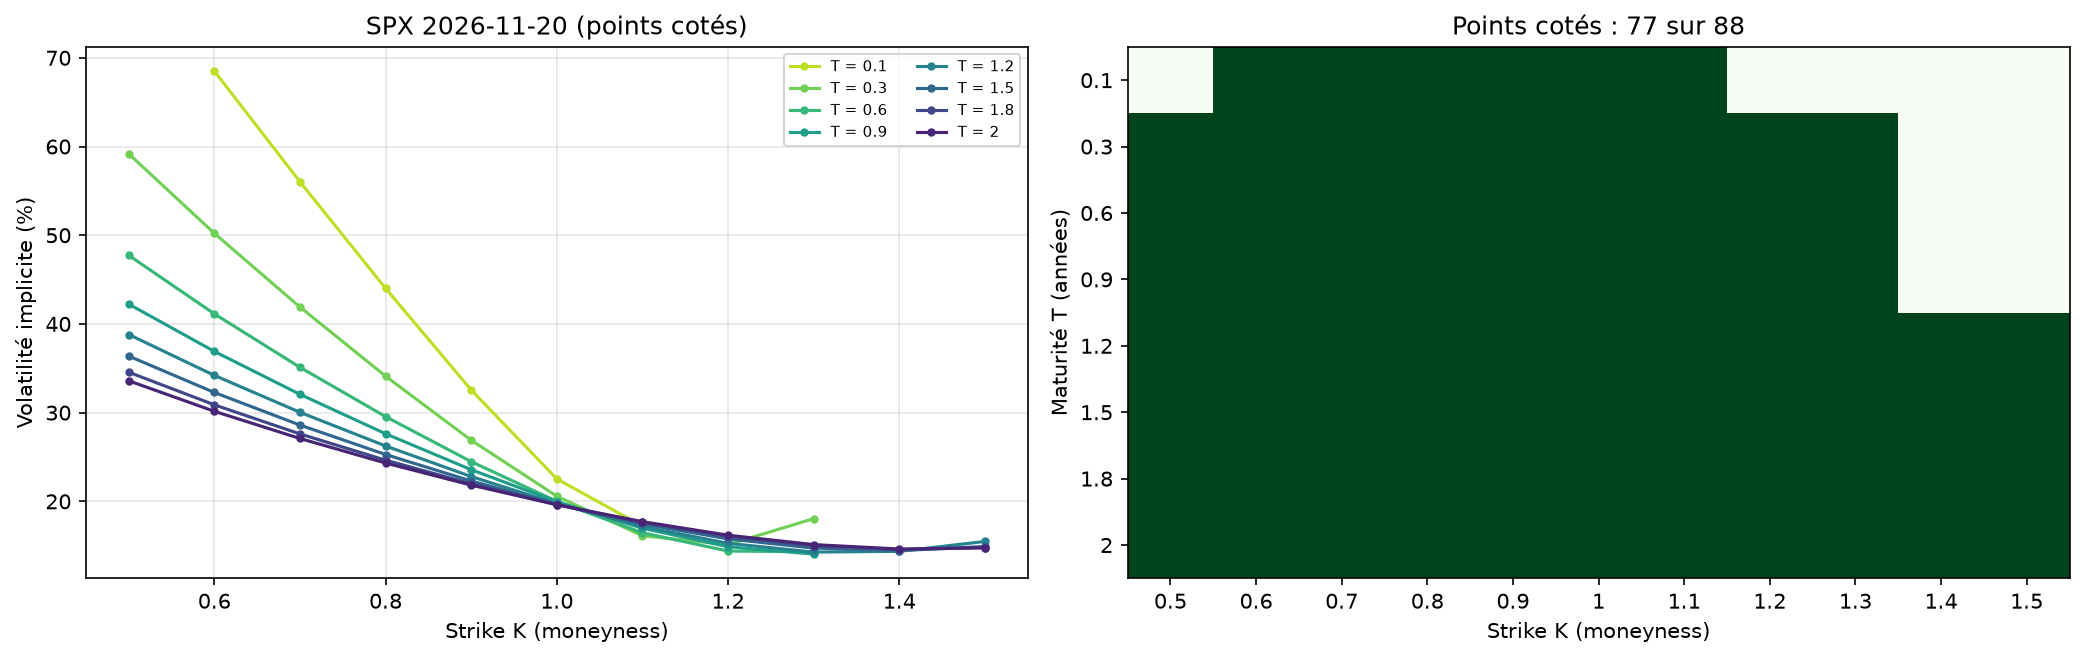
\includegraphics[width=\textwidth]{etape0_spx}
  \caption{Surface SPX du dernier jour collecté (points cotés seulement) et masque des points cotés.}
  \label{fig-spx}
\end{figure}

\paragraph{La zone de calibration.} Le skew du SPX à court terme est extrêmement raide : le 4 novembre, à un mois,
la volatilité valait \SI{13.4}{\percent} à la monnaie mais \SI{71.7}{\percent} pour $K = 0{,}5$. Le modèle de
Heston, sans sauts, ne peut pas produire une telle pente sur une maturité aussi courte. C'est une limite connue,
qui motive notamment les modèles à volatilité rugueuse étudiés par \citet{horvath2021}. Calibré sur tous les points
cotés, Heston fait de \SI{100}{\pb} à \SI{170}{\pb} d'erreur moyenne selon les jours, jusqu'à 20 points de
volatilité sur certains points, et ses paramètres partent vers des valeurs extrêmes (sans borne, $\xi \approx 4$ à 5
et un ratio de Feller proche de \num{0.05}). Nous calibrons donc sur la zone liquide,
proche de la monnaie : strikes de \num{0.7} à \num{1.3} et maturités d'au moins \num{0.3} an (49 points de la grille,
réglage \texttt{spx\_calibration} de \texttt{base.yaml}). Les autres points restent dans les données mais ne servent
pas à calibrer.

\paragraph{Calibration d'essai.} Avant l'étape~4, nous avons calibré les quatre jours avec le pricer Fourier et le
même optimiseur que l'étape~4 (Levenberg-Marquardt, cinq points de départ), sur cette zone
(\cref{tab-spx-calibration}, \cref{fig-spx-calibration}).

\begin{table}[H]
  \centering
  \caption{Calibration de Heston sur les surfaces SPX (pricer Fourier, zone de calibration). Erreurs en points de
  base ; « tous » : erreur moyenne sur tous les points cotés, pour comparaison.}
  \label{tab-spx-calibration}
  \begin{tabular}{lrrrrrrrr}
    \toprule
    Date & $v_0$ & $\theta$ & $\kappa$ & $\xi$ & $\rho$ & Feller & Zone (moy.~/ max) & Tous \\
    \midrule
    3 nov.  & \num{0.036} & \num{0.049} & \num{3.89} & \num{1.5} & \num{-0.72} & \num{0.17} & \num{29.2} / 146 & 98 \\
    4 nov.  & \num{0.023} & \num{0.049} & \num{3.99} & \num{1.5} & \num{-0.71} & \num{0.17} & \num{29.5} / 125 & 120 \\
    5 nov.  & \num{0.053} & \num{0.050} & \num{3.82} & \num{1.5} & \num{-0.75} & \num{0.17} & \num{29.1} / 165 & 141 \\
    20 nov. & \num{0.076} & \num{0.055} & \num{3.89} & \num{1.5} & \num{-0.76} & \num{0.19} & \num{29.8} / 123 & 94 \\
    \bottomrule
  \end{tabular}
\end{table}

Les paramètres sont stables d'un jour à l'autre ($\kappa \approx 3{,}9$, $\theta \approx 0{,}05$,
$\rho \approx -0{,}73$), et $v_0$ suit la volatilité de court terme du marché. Tous restent dans le domaine
d'entraînement (ratio de Feller entre \num{0.17} et \num{0.19}), à une exception près : $\xi$ atteint sa borne de
\num{1.5} les quatre jours. Sans borne, il vaudrait environ 2, pour la même erreur moyenne. Élargir le domaine à
$\xi \leq 2{,}5$ ne rendrait pas les grandes zones utilisables (l'obstacle est la maturité d'un mois) et pousserait
le ratio de Feller vers \num{0.1}, au bord du domaine appris : nous avons gardé $\xi \leq 1{,}5$.

\begin{figure}[H]
  \centering
  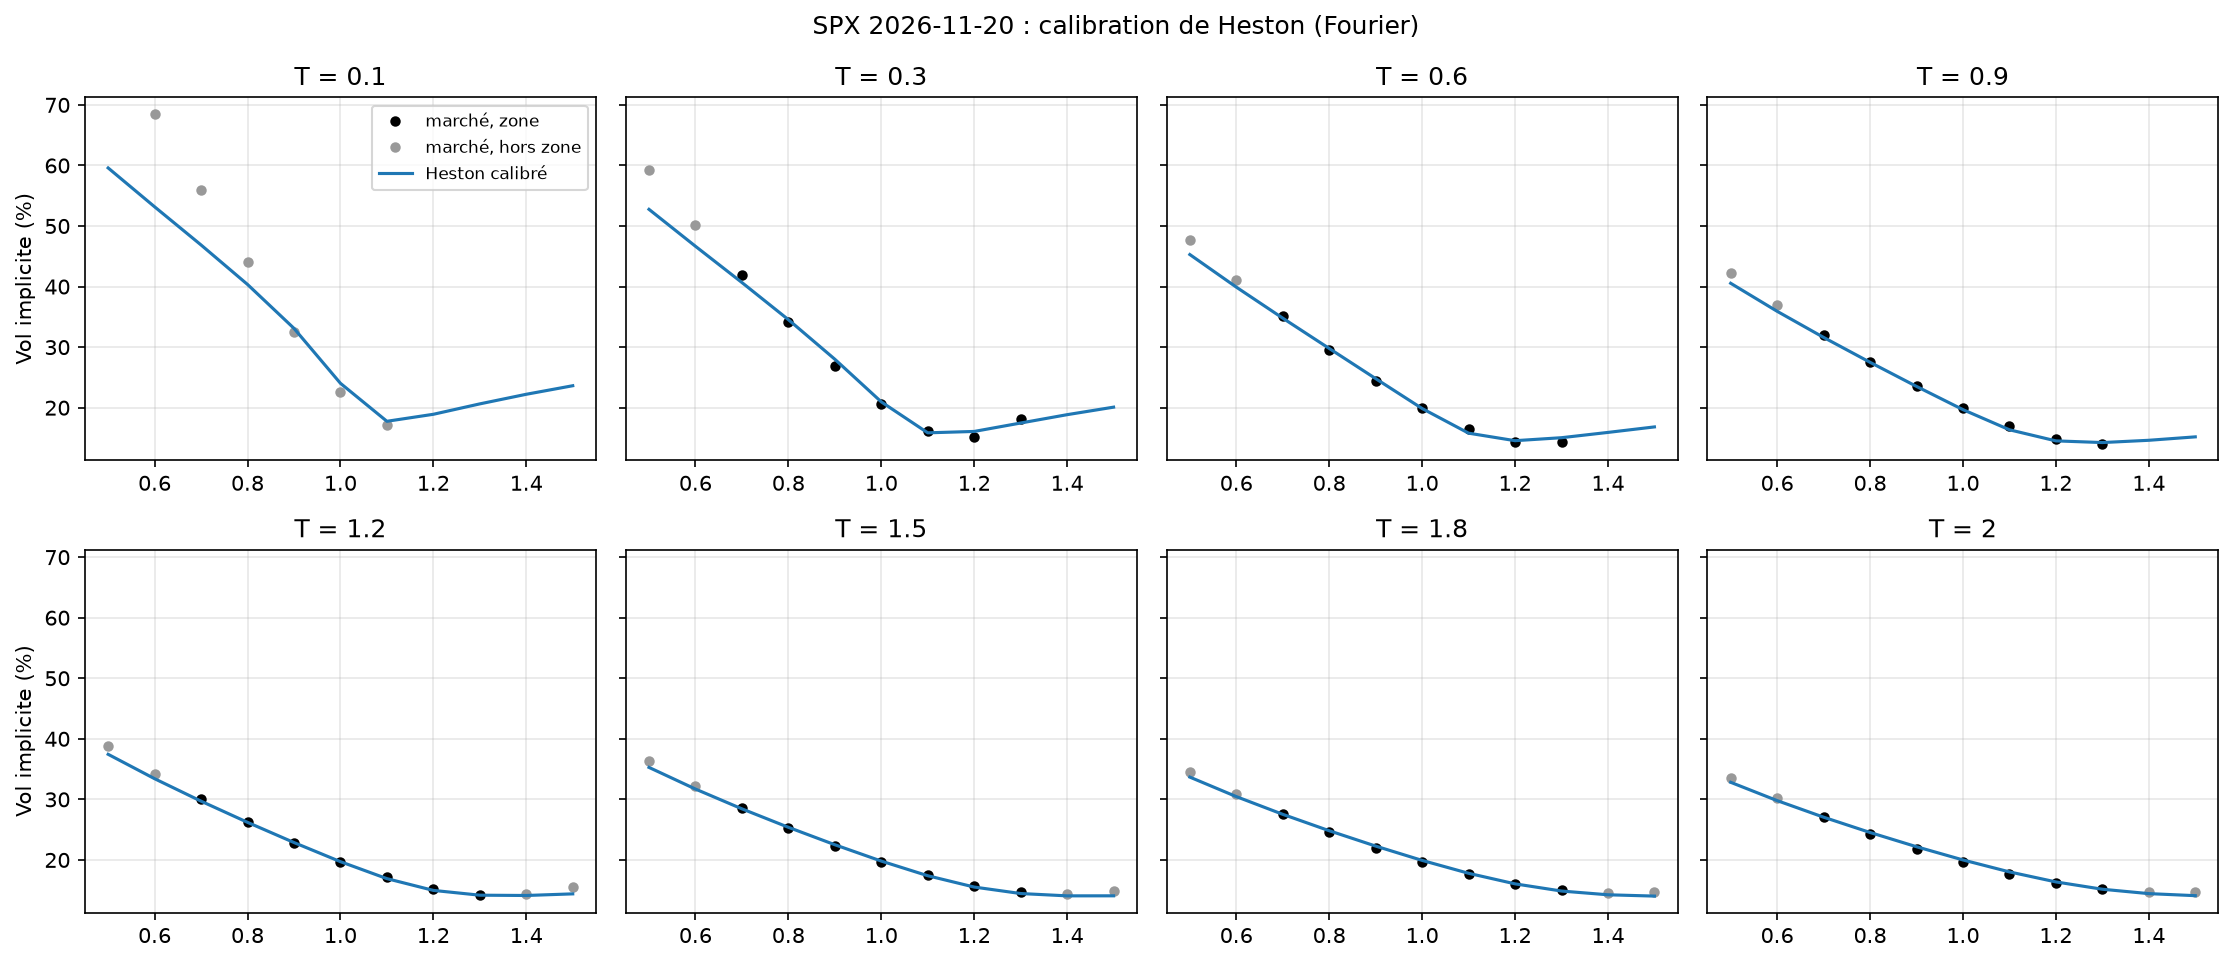
\includegraphics[width=\textwidth]{etape0_spx_calibration}
  \caption{Calibration du 20 novembre, maturité par maturité : points du marché dans la zone (noirs) et hors zone
  (gris), et Heston calibré (trait).}
  \label{fig-spx-calibration}
\end{figure}

\subsection{Limites}
\label{sec-limites-donnees}

\begin{itemize}
  \item Nous avons peu de jours de marché, tous dans le même régime. Yahoo Finance ne fournit pas d'historique :
  nos surfaces SPX couvrent quelques jours de novembre 2026, avec une volatilité entre \SI{13}{\percent} et
  \SI{23}{\percent}. Elles montrent la calibration sur données réelles, mais ne disent rien d'un marché très calme
  ou en crise. Il faudrait pour cela une base historique (OptionMetrics, par exemple).
  \item La surface de marché a sa propre imprécision, due au lissage SVI : environ \SI{8}{\pb} en moyenne sur des
  données fictives, plus avec le bruit réel. C'est du même ordre que l'erreur du réseau.
  \item Sur le SPX, $\xi$ atteint sa borne, et Heston ne peut pas reproduire le skew à un mois : nous calibrons
  sur une zone réduite de la surface.
\end{itemize}

% Organisation du code et des calculs.

\section{Mise en œuvre}
\label{sec-mise-en-oeuvre}

Les expériences des sections suivantes demandent plus d'une centaine d'entraînements, dont certains durent près
d'une heure. Nous avons donc organisé le code et les calculs pour pouvoir corriger, relancer et partager le travail
sans rien recalculer inutilement.

\subsection{Un code modulaire}

Tout le code réutilisable est regroupé dans un paquet Python (\texttt{src/heston\_nn}), découpé par rôle :
chargement et découpage des données, construction du réseau, entraînement, métriques, calibration et figures.
Les notebooks restent courts : ils appellent ces fonctions et présentent les résultats. Les règles communes
(grille, plages des paramètres, découpage, budget d'entraînement, graines) sont écrites une seule fois dans un
fichier de configuration (\texttt{configs/base.yaml}) ; chaque expérience n'a qu'un petit fichier qui précise ce
qui change (par exemple l'activation).

Cette organisation nous a permis de corriger et d'améliorer le code tout au long du projet sans toucher aux
notebooks : une correction dans une fonction profite à toutes les étapes. Par exemple, la gestion des points
manquants (NaN) dans la perte a été ajoutée une seule fois, dans la fonction d'entraînement, et s'applique à tous
les réseaux. Une centaine de tests automatiques vérifient chaque fonction sur des données de petite taille, ce qui
a permis de repérer les erreurs avant de lancer les longs calculs.

\subsection{Des calculs partagés et enregistrés}

Pour aller plus vite, les entraînements sont répartis entre nos 4 machines. Chaque membre de l'équipe a un numéro
de machine (de 0 à 3) : la liste de toutes les expériences, c'est-à-dire chaque configuration avec chaque graine,
est partagée de façon que chaque machine en prenne une sur quatre. Il suffit de changer ce numéro dans le notebook
pour que chacun calcule sa part.

Chaque entraînement terminé est enregistré dans son propre dossier, un par configuration et par graine :
les erreurs, l'historique d'apprentissage et le réseau. Avant de lancer un entraînement, le code vérifie s'il est
déjà fait ; si oui, il relit simplement le résultat. Un calcul n'est donc fait qu'une seule fois : si une machine
s'arrête en cours de route, il suffit de relancer la même cellule pour reprendre là où elle en était. Les résultats
de chaque machine sont ensuite rassemblés sur GitHub, et le notebook les relit tous pour tracer les courbes et
faire les tableaux. Une même référence n'est jamais recalculée : le réseau retenu à l'étape 1 sert directement de
référence à l'étape 2.

\subsection{Reproductibilité}

Toutes les sources de hasard sont fixées par une graine : tirage des paramètres, découpage des données,
initialisation des poids et ordre des lots. Avec la même configuration et la même graine, un entraînement redonne
les mêmes résultats. Le code, les configurations, les données d'entraînement et les résultats sont versionnés sur
GitHub, de sorte que chaque chiffre de ce rapport peut être retrouvé et recalculé.

% Étape 1 : choix de l'architecture. Sources : notebooks/01_architectures.ipynb, results/etape1_*.

\section{Choix de l'architecture}
\label{sec-architectures}

Le réseau doit remplacer Fourier pendant la calibration : il doit donc être à la fois précis et nettement plus
rapide que Fourier. Cette section choisit sa taille, c'est-à-dire le nombre de couches cachées et de neurones par
couche.

\subsection{Protocole}
\label{sec-archi-protocole}

Le réseau est un perceptron multicouche : il prend les 5 paramètres de Heston (normalisés) et renvoie les 88
volatilités de la grille ; la couche de sortie est linéaire, puisqu'il s'agit d'une régression. La perte est
l'erreur quadratique moyenne, calculée uniquement sur les points connus de chaque surface : les points manquants
(NaN, voir \cref{sec-donnees}) sont ignorés, ce qui permet de garder toutes les surfaces.

Nous comparons 10 architectures : 2, 4 ou 6 couches cachées de 32, 128 ou 512 neurones, plus le réseau
$4\times30$ de \citet{horvath2021}, qui sert de référence. Seule l'architecture change : toutes sont entraînées
de la même façon, avec Adam, l'initialisation de He et l'activation ELU, pendant 200 époques avec des lots de 32
surfaces, sur le même découpage des données (\SI{80}{\percent} entraînement, \SI{10}{\percent} validation,
\SI{10}{\percent} test). Nous gardons les poids de la meilleure époque sur la validation.

Chaque architecture est entraînée 5 fois, avec 5 graines différentes, sur exactement le même découpage des
données : la graine ne change que l'initialisation des poids et l'ordre des lots. Les écarts-types mesurent donc
la variabilité de l'entraînement lui-même, pas celle des données. Les choix se font sur la validation ; le test ne
sert qu'aux chiffres finaux. L'erreur est l'écart absolu moyen entre la volatilité prédite et la vraie, en points
de base ($1\pb = 0{,}01$ point de volatilité).

\subsection{Taux d'apprentissage}
\label{sec-archi-taux}

Avant de comparer les architectures, nous fixons le taux d'apprentissage d'Adam sur le réseau de référence
$4\times30$, avec trois valeurs (\cref{fig-taux}). Avec $10^{-2}$, l'apprentissage est instable : l'erreur de
validation oscille et atteint \num{14.3}\pb. Avec $10^{-4}$, il est trop lent : \num{9.2}\pb\ après 200 époques,
et le réseau progresse encore. Nous retenons $10^{-3}$ (\num{7.6}\pb), utilisé dans toute la suite.

\begin{figure}[H]
  \centering
  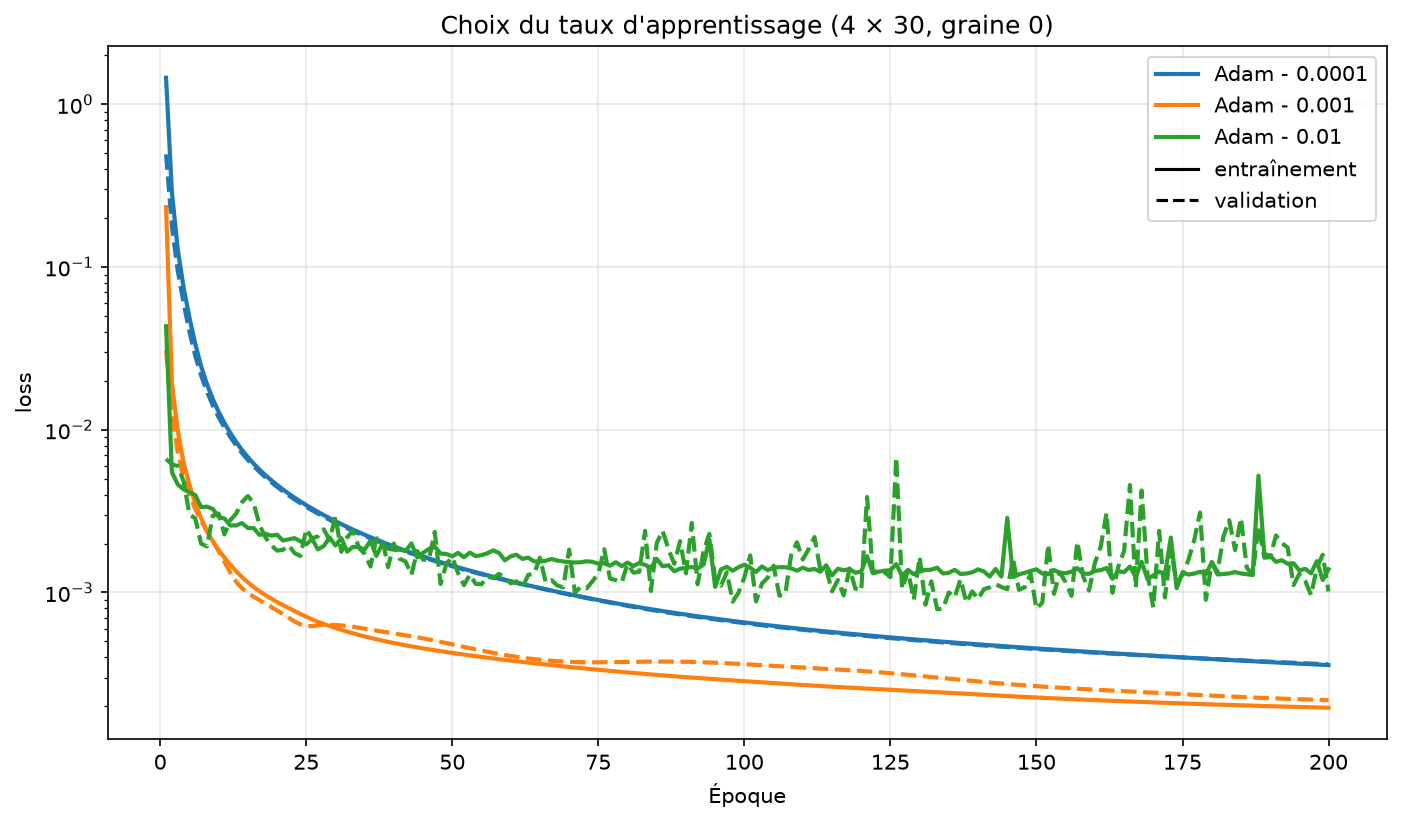
\includegraphics[width=0.8\textwidth]{etape1_taux}
  \caption{Perte d'entraînement (trait plein) et de validation (pointillés) du réseau $4\times30$ pour trois taux
  d'apprentissage.}
  \label{fig-taux}
\end{figure}

\subsection{Précision}
\label{sec-archi-precision}

Le \cref{tab-archi} donne les erreurs des 10 architectures et la \cref{fig-courbes} leurs courbes
d'apprentissage.

Augmenter la taille du réseau n'améliore pas la précision au-delà d'un certain point. Les réseaux de 512 neurones
sur 4 et 6 couches sont moins précis que des réseaux bien plus petits, et instables d'une graine à l'autre : le
$6\times512$ fait \num{14.8} $\pm$ \num{11.5}\pb. Leur perte de validation reste au-dessus des autres et oscille
fortement (\cref{fig-courbes}), signe qu'avec le même taux d'apprentissage, ces grands réseaux sont plus difficiles
à entraîner.

Ajouter des couches n'aide pas non plus. À largeur constante de 128 neurones, les réseaux plus profonds font même
un peu moins bien (\num{5.09},
\num{5.45} et \num{5.90}\pb\ pour 2, 4 et 6 couches). À 32 neurones, toutes les profondeurs se valent (de
\num{6.5} à \num{7.6}\pb), et le réseau de \citet{horvath2021} se situe au même niveau (\num{6.75}\pb).

Les erreurs de validation et de test sont très proches pour toutes les architectures : l'écart absolu moyen est
de \num{0.04}\pb, et ne dépasse jamais \num{0.2}\pb. Les deux jeux sont pourtant distincts et évalués séparément :
leurs erreurs maximales diffèrent nettement (pour le $2\times128$, graine 0 : \num{112}\pb\ en validation contre
\num{129}\pb\ en test). Cette proximité s'explique par leur taille : chacun contient \num{5000} surfaces, soit
environ \num{430000} volatilités connues tirées de la même distribution, ce qui stabilise l'estimation de l'erreur
moyenne, même si les volatilités d'une même surface ne sont pas indépendantes. À la meilleure époque, la perte
d'entraînement reste du même ordre que la perte de validation : nous ne voyons pas de surapprentissage marqué.
La meilleure époque est le plus souvent entre 170 et 200 :
avec un budget plus long, les réseaux progresseraient encore un peu.

\begin{table}[H]
  \centering
  \caption{Erreur moyenne (pb, moyenne $\pm$ écart-type sur 5 graines), erreur maximale moyenne sur le test,
  nombre de paramètres, temps de réponse pour une surface et gain par rapport à Fourier (\SI{2.29}{\ms}).
  Les erreurs de validation et de test diffèrent de moins de 0,2 pb, d'où des valeurs identiques une fois
  arrondies.}
  \label{tab-archi}
  \small
  \begin{tabular}{lcccrrr}
    \toprule
    Architecture & Validation & Test & Erreur max & Paramètres & Temps (ms) & Gain \\
    \midrule
    $2\times512$          & $4{,}67 \pm 0{,}42$   & $4{,}67$  & 173 & \num{310872}  & \num{0.39}  & \num{5.9} \\
    $\mathbf{2\times128}$ & $\mathbf{5{,}09 \pm 0{,}52}$ & $\mathbf{5{,}09}$ & 161 & \num{28632} & \num{0.028} & \num{83} \\
    $4\times128$          & $5{,}45 \pm 0{,}33$   & $5{,}45$  & 145 & \num{61656}   & \num{0.051} & \num{45} \\
    $6\times128$          & $5{,}90 \pm 0{,}26$   & $5{,}89$  & 132 & \num{94680}   & \num{0.074} & \num{31} \\
    $4\times32$           & $6{,}52 \pm 1{,}07$   & $6{,}49$  & 164 & \num{6264}    & \num{0.023} & \num{99} \\
    $4\times30$ (Horvath) & $6{,}75 \pm 0{,}67$   & $6{,}77$  & 150 & \num{5698}    & \num{0.023} & \num{100} \\
    $6\times32$           & $6{,}75 \pm 0{,}78$   & $6{,}78$  & 145 & \num{8376}    & \num{0.032} & \num{72} \\
    $2\times32$           & $7{,}63 \pm 0{,}86$   & $7{,}64$  & 249 & \num{4152}    & \num{0.020} & \num{113} \\
    $4\times512$          & $7{,}90 \pm 1{,}20$   & $7{,}90$  & 145 & \num{836184}  & \num{1.18}  & \num{1.9} \\
    $6\times512$          & $14{,}8 \pm 11{,}5$   & $14{,}8$  & 241 & \num{1361496} & \num{2.11}  & \num{1.1} \\
    \bottomrule
  \end{tabular}
\end{table}

\begin{figure}[H]
  \centering
  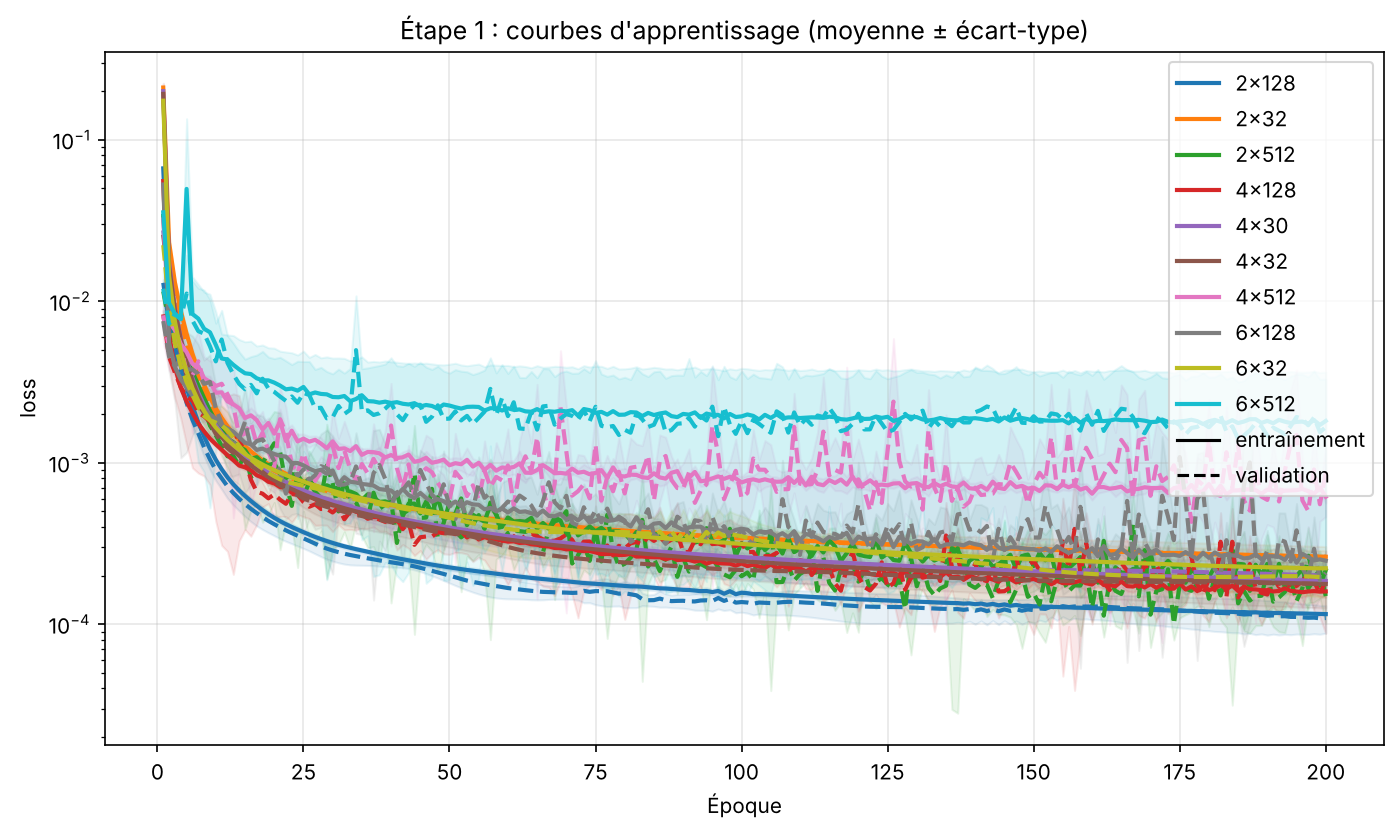
\includegraphics[width=\textwidth]{etape1_courbes}
  \caption{Courbes d'apprentissage des 10 architectures : moyenne $\pm$ écart-type sur 5 graines, entraînement en
  trait plein et validation en pointillés.}
  \label{fig-courbes}
\end{figure}

\subsection{Temps de réponse et choix}
\label{sec-archi-choix}

Le temps de réponse est mesuré pour une seule surface, sur la même machine que Fourier, au repos. Pour une seule
surface, un appel à Keras ajoute environ \SI{3}{\ms} de frais fixes, plus que Fourier lui-même : nous mesurons donc
la prédiction refaite en numpy, couche par couche, à partir des poids du réseau. Ce temps ne dépend que de la
taille du réseau, et grandit vite avec la largeur : de \SI{0.02}{\ms} pour les réseaux de 32 neurones à
\SI{2.1}{\ms} pour le $6\times512$, presque autant que Fourier.

Le seuil de vitesse a été fixé en regardant uniquement les temps, avant de comparer les précisions : le réseau doit
être au moins 10 fois plus rapide que Fourier. Il élimine les trois réseaux de 512 neurones, entre 1,1 et
5,9 fois plus rapides seulement (\cref{fig-erreur-temps}). Pour choisir parmi les 7 architectures restantes, nous
partons de la plus précise sur la validation ; comme l'écart entre deux architectures reste faible au regard de la
variabilité observée entre les graines, nous retenons la plus rapide de celles qui sont à moins d'un écart-type
d'elle. La plus précise est le $2\times128$ (\num{5.09} $\pm$ \num{0.52}\pb) ; le $4\times128$ est à moins d'un
écart-type (\num{5.45}\pb), mais presque deux fois plus lent.

Nous retenons donc le $2\times128$ : \num{5.09}\pb\ sur la validation et sur le test, 83 fois plus rapide que
Fourier. Il fait mieux que l'architecture $4\times30$ de \citet{horvath2021}, entraînée avec notre protocole
(\num{6.75}\pb), pour un temps de réponse comparable.

\begin{figure}[H]
  \centering
  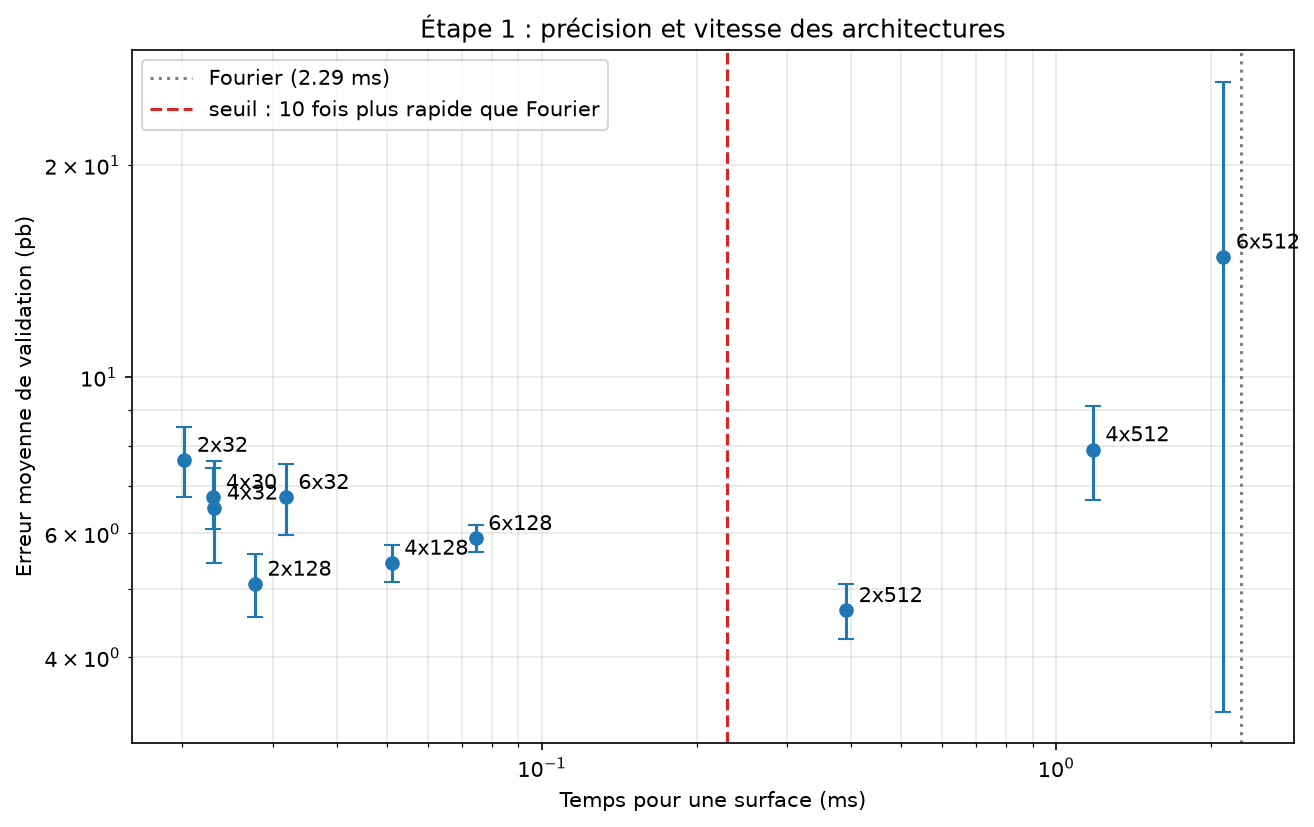
\includegraphics[width=0.85\textwidth]{etape1_erreur_temps}
  \caption{Erreur de validation (moyenne $\pm$ écart-type sur 5 graines) en fonction du temps de réponse pour une
  surface. Ligne pointillée grise : Fourier ; ligne rouge : seuil de vitesse (10 fois plus rapide que Fourier).}
  \label{fig-erreur-temps}
\end{figure}

% Étape 2 : choix de l'entraînement. Sources : notebooks/02_choix_entrainement.ipynb, results/etape2_*.

\section{Choix de l'entraînement}
\label{sec-entrainement}

L'architecture est maintenant fixée ($2\times128$). Nous cherchons comment l'entraîner au mieux, en comparant
les choix vus en cours : l'optimiseur, l'initialisation des poids et la fonction d'activation.

\subsection{Protocole}
\label{sec-entr-protocole}

Nous changeons un seul élément à la fois par rapport à la référence de l'étape 1 : Adam, initialisation de He,
activation ELU (\cref{tab-comparaisons}). Le reste de l'entraînement ne change pas : 200 époques, lots de 32
surfaces, même découpage des données. Comme à l'étape 1, les graines ne changent que l'initialisation des poids
et l'ordre des lots.

\begin{table}[H]
  \centering
  \caption{Les trois comparaisons. La référence est en gras.}
  \label{tab-comparaisons}
  \small
  \begin{tabular}{lll}
    \toprule
    Comparaison & Ce qui varie & Reste fixe \\
    \midrule
    Optimiseurs      & SGD, moment, AdaGrad, RMSProp, \textbf{Adam} & He + ELU \\
    Initialisations  & naïve, Xavier, \textbf{He}                   & Adam + ELU \\
    Activations      & \textbf{ELU}, ReLU, tanh, sigmoïde, GELU, SiLU, linéaire & Adam + He \\
    \bottomrule
  \end{tabular}
\end{table}

Pour que les calculs restent réalisables dans le temps du projet, nous avons allégé cette étape de trois façons.
Chaque configuration est entraînée avec 3 graines au lieu de 5. Le taux d'Adam n'est pas réglé à nouveau : nous
gardons $10^{-3}$, choisi à l'étape 1. Enfin, Leaky ReLU n'est pas testée, afin de limiter le nombre de
configurations. L'étape passe ainsi d'environ 90 à environ 50 entraînements.

La configuration de référence (Adam + He + ELU) est exactement le réseau retenu à l'étape 1 : nous reprenons les
résultats de ses graines 0, 1 et 2, les mêmes graines que pour les autres configurations de cette étape. Sa
moyenne sur ces 3 graines (\num{5.11} $\pm$ \num{0.71}\pb) diffère donc légèrement de celle sur les 5 graines de
l'étape 1 (\num{5.09} $\pm$ \num{0.52}\pb).

\subsection{Réglage du taux de chaque optimiseur}
\label{sec-entr-taux}

Chaque optimiseur a son propre bon taux d'apprentissage. Pour comparer des optimiseurs bien réglés, nous
entraînons chacun avec trois taux, sur une graine (\cref{tab-taux-optim}).

\begin{table}[H]
  \centering
  \caption{Erreur moyenne de validation (pb) selon l'optimiseur et le taux d'apprentissage (une graine).
  Le meilleur taux de chaque optimiseur est en gras.}
  \label{tab-taux-optim}
  \begin{tabular}{lccc}
    \toprule
    Optimiseur & $10^{-4}$ & $10^{-3}$ & $10^{-2}$ \\
    \midrule
    RMSProp & \num{9.7}   & $\mathbf{5{,}6}$ & \num{28.3} \\
    Moment  & \num{70.0}  & \num{32.0}  & $\mathbf{11{,}4}$ \\
    AdaGrad & \num{155.3} & \num{58.7}  & $\mathbf{21{,}3}$ \\
    SGD     & \num{139.0} & \num{70.0}  & $\mathbf{32{,}1}$ \\
    \bottomrule
  \end{tabular}
\end{table}

Le taux compte autant que l'optimiseur. RMSProp passe de \num{5.6} à \num{28.3}\pb\ si le taux est trop grand.
SGD, le moment et AdaGrad, au contraire, sont meilleurs avec le plus grand taux testé : avec un taux plus petit, ils
avancent trop lentement et n'ont pas convergé en 200 époques. Leur meilleur taux étant au bord de la grille, un taux
plus grand pourrait encore les améliorer ; c'est une limite de notre réglage.

\subsection{Résultats}
\label{sec-entr-resultats}

Le \cref{tab-entrainement} donne les erreurs de toutes les configurations et la \cref{fig-comparaisons} leurs
courbes d'apprentissage. Comme à l'étape 1, les erreurs de validation et de test restent très proches (écart
absolu moyen de \num{0.04}\pb, au plus \num{0.18}\pb).

\begin{table}[H]
  \centering
  \caption{Erreur moyenne (pb, moyenne $\pm$ écart-type sur 3 graines) pour chaque comparaison. La référence
  (Adam + He + ELU) est la même dans les trois comparaisons.}
  \label{tab-entrainement}
  \small
  \begin{tabular}{llcc}
    \toprule
    Comparaison & Configuration & Validation & Test \\
    \midrule
    Optimiseurs     & Adam (référence)  & $5{,}11 \pm 0{,}71$ & $5{,}10$ \\
                    & RMSProp           & $5{,}93 \pm 1{,}06$ & $5{,}93$ \\
                    & Moment            & $11{,}4 \pm 0{,}2$  & $11{,}5$ \\
                    & AdaGrad           & $21{,}3 \pm 0{,}2$  & $21{,}4$ \\
                    & SGD               & $32{,}3 \pm 0{,}2$  & $32{,}4$ \\
    \midrule
    Initialisations & Xavier            & $5{,}04 \pm 0{,}39$ & $5{,}03$ \\
                    & He (référence)    & $5{,}11 \pm 0{,}71$ & $5{,}10$ \\
                    & Naïve             & $5{,}31 \pm 0{,}24$ & $5{,}31$ \\
    \midrule
    Activations     & GELU              & $\mathbf{2{,}66 \pm 0{,}09}$ & $\mathbf{2{,}67}$ \\
                    & SiLU              & $2{,}75 \pm 0{,}20$ & $2{,}73$ \\
                    & Sigmoïde          & $4{,}24 \pm 0{,}20$ & $4{,}25$ \\
                    & tanh              & $5{,}05 \pm 0{,}60$ & $5{,}05$ \\
                    & ELU (référence)   & $5{,}11 \pm 0{,}71$ & $5{,}10$ \\
                    & ReLU              & $6{,}16 \pm 0{,}99$ & $6{,}19$ \\
                    & Linéaire (témoin) & $156 \pm 1$         & $155$ \\
    \bottomrule
  \end{tabular}
\end{table}

\begin{figure}[H]
  \centering
  \begin{subfigure}{\textwidth}
    \centering
    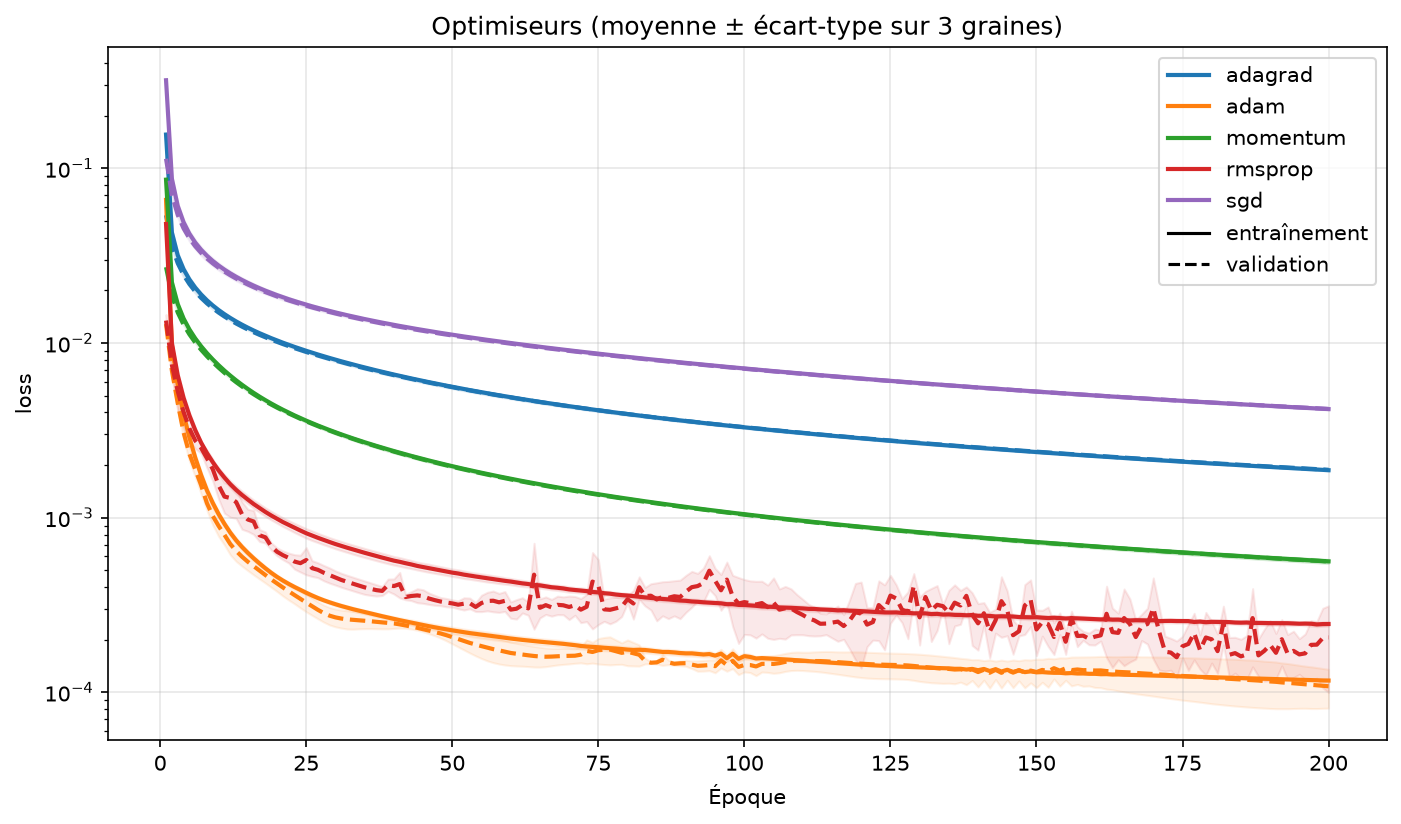
\includegraphics[width=0.62\textwidth]{etape2_serieA}
    \caption{Optimiseurs.}
  \end{subfigure}
  \begin{subfigure}{\textwidth}
    \centering
    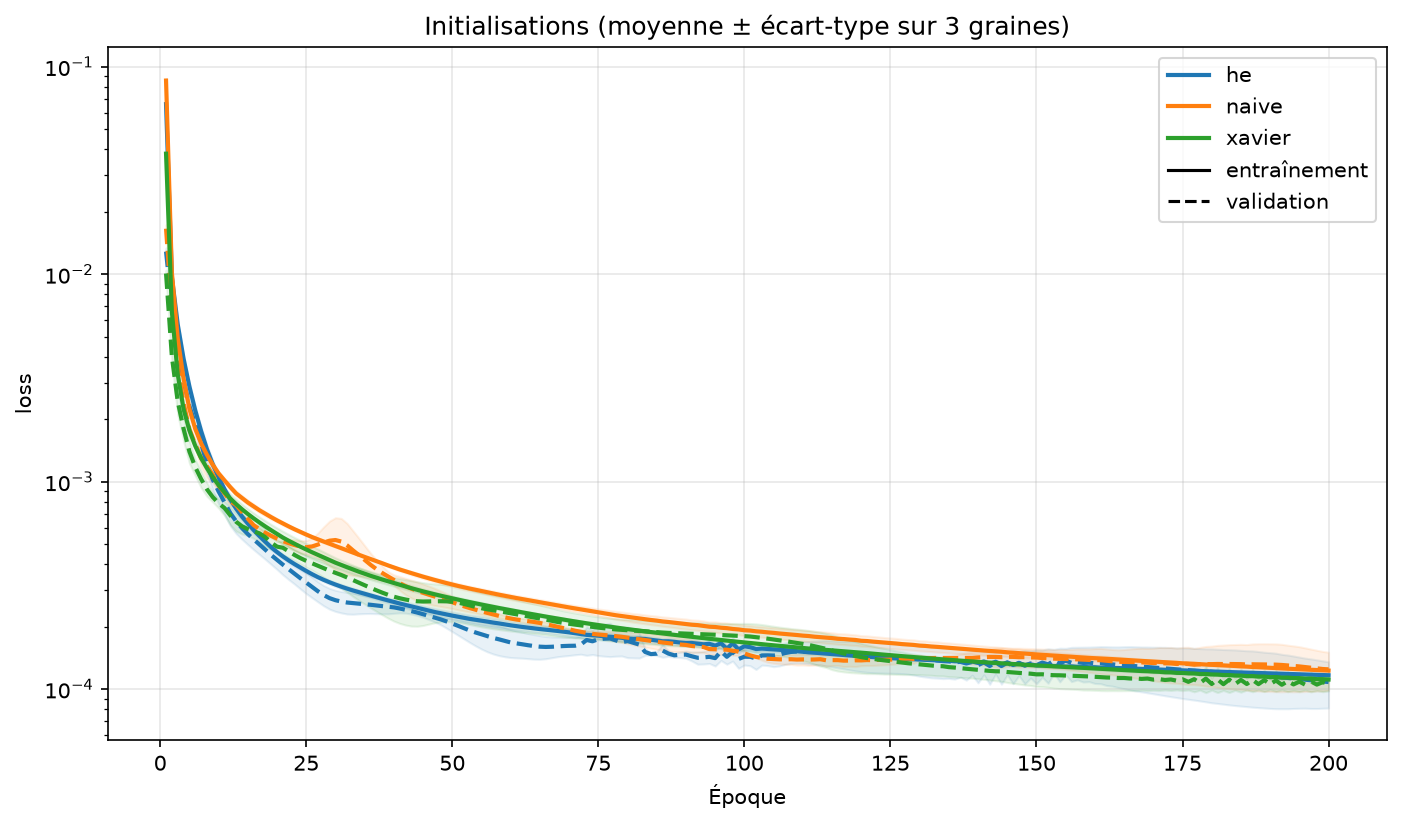
\includegraphics[width=0.62\textwidth]{etape2_serieB}
    \caption{Initialisations.}
  \end{subfigure}
  \begin{subfigure}{\textwidth}
    \centering
    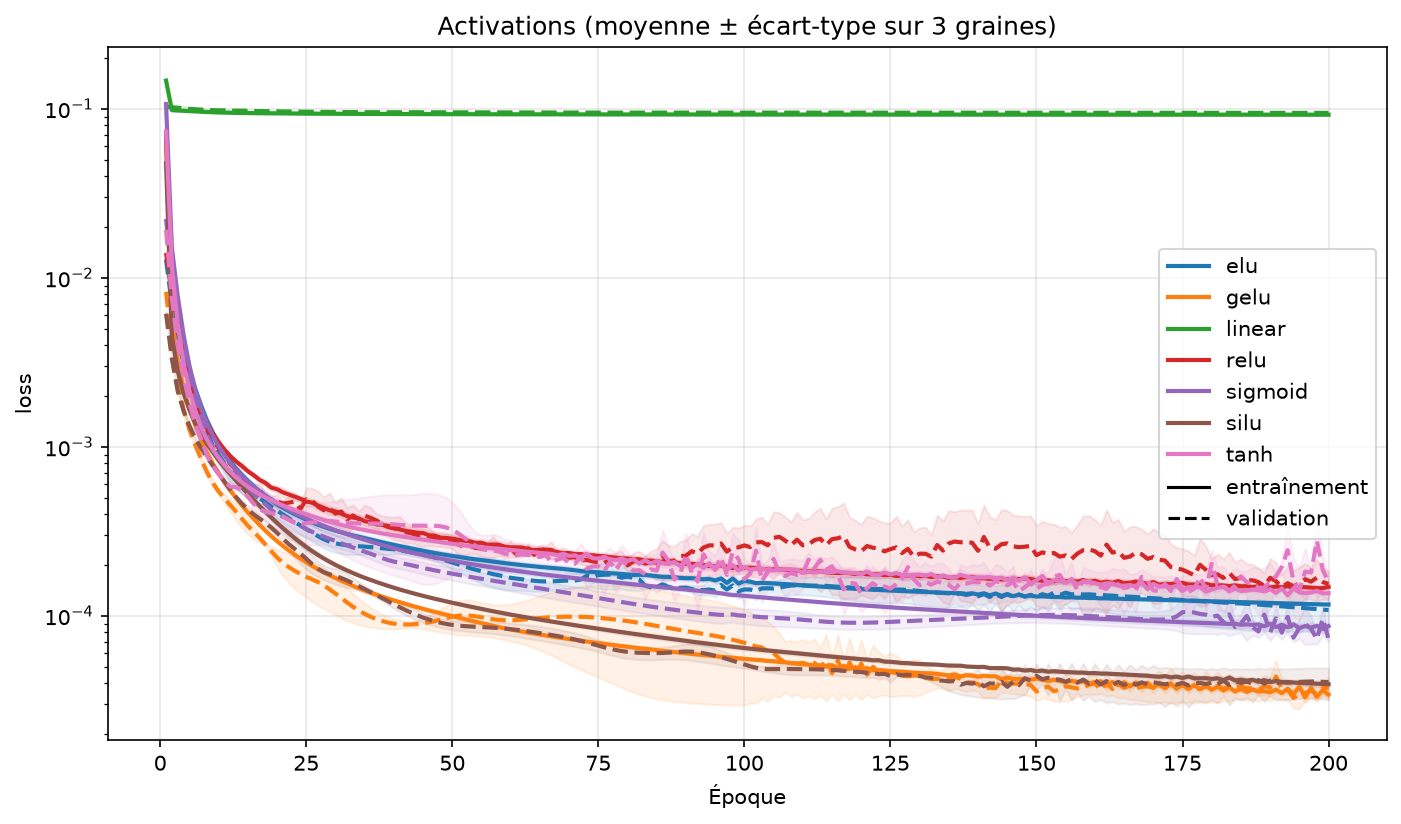
\includegraphics[width=0.62\textwidth]{etape2_serieC}
    \caption{Activations.}
  \end{subfigure}
  \caption{Courbes d'apprentissage : moyenne $\pm$ écart-type sur 3 graines, entraînement en trait plein et
  validation en pointillés.}
  \label{fig-comparaisons}
\end{figure}

C'est l'activation qui fait la plus grande différence dans nos expériences. GELU obtient la meilleure moyenne
observée (\num{2.66}\pb), devant SiLU (\num{2.75}\pb) ; avec 3 graines et ces écarts-types, nous ne pouvons pas
départager ces deux activations. Toutes deux divisent l'erreur par deux par rapport à ELU (\num{5.11}\pb) et font
bien mieux que ReLU (\num{6.16}\pb). Leur caractère lisse pourrait favoriser une approximation régulière de la
surface de volatilité, dont les variations sont elles-mêmes continues ; cette explication reste une interprétation,
que notre expérience ne permet pas d'isoler. Le témoin linéaire, lui, échoue (\num{156}\pb) : sans
non-linéarité, le réseau se réduit à une régression linéaire et ne peut pas représenter la surface.

L'optimiseur compte aussi beaucoup. Adam et RMSProp sont les meilleurs des optimiseurs testés ; le moment, AdaGrad
et SGD restent 2 à 6 fois moins précis, même après réglage de leur taux d'apprentissage. L'initialisation, en revanche, compte peu pour ce réseau de 2 couches :
les trois initialisations sont à moins d'un écart-type les unes des autres.

\subsection{Réseau final}
\label{sec-entr-final}

Nous combinons d'abord le meilleur réglage de chaque comparaison : Adam, initialisation Xavier, activation GELU.
Ces choix ayant été testés un par un, nous vérifions qu'ensemble ils font mieux que la référence. Ce n'est pas le
cas : la combinaison fait \num{2.91} $\pm$ \num{0.14}\pb, moins bien que GELU avec l'initialisation He
(\num{2.66} $\pm$ \num{0.09}\pb). Les meilleurs choix ne s'additionnent donc pas : dans nos expériences, Xavier
est un peu meilleure que He avec ELU, mais la combinaison He + GELU obtient une meilleure moyenne que
Xavier + GELU. Les hyperparamètres interagissent : le meilleur réglage d'un élément dépend des autres.

Le réseau final est le $2\times128$ entraîné avec Adam ($10^{-3}$), l'initialisation de He et l'activation GELU :
\num{2.66}\pb\ sur la validation et \num{2.67}\pb\ sur le test en moyenne sur 3 graines, soit deux fois moins
d'erreur que la référence de l'étape 1, pour le même temps de réponse. Nous gardons la graine la plus précise sur
la validation (\num{2.58}\pb\ sur le test) ; c'est ce réseau qui sert dans la suite.

% Étape 3 : réseau contre ML classique. Sources : notebooks/03_dl_vs_ml.ipynb, results/etape3/,
% results/etape3_reseau_final_sans_nan/, results/etape3_courbe_*/, results/figures/etape3_courbe_apprentissage.png.

\section{Réseau de neurones contre apprentissage classique}
\label{sec-dl-vs-ml}

Un réseau de neurones est-il nécessaire pour cette tâche ? Pour répondre, nous entraînons cinq modèles classiques
de scikit-learn sur la même tâche (5 paramètres de Heston, 88 volatilités) et les comparons au réseau final de la
\cref{sec-entrainement}, avec les mêmes métriques : précision sur le test, temps de réponse pour une surface et
évolution de l'erreur avec la taille du jeu d'entraînement.

\subsection{Protocole}
\label{sec-ml-protocole}

\paragraph{Les modèles.} Nous testons une régression ridge sur des monômes des paramètres, les $k$ plus proches
voisins, une forêt aléatoire, LightGBM (un modèle par volatilité, soit 88 modèles) et un processus gaussien (GP)
à noyau RBF avec un terme de bruit. Les hyperparamètres sont choisis sur la validation, dans les petites grilles du
\cref{tab-ml-grilles}. Les paramètres d'entrée sont normalisés avec la moyenne et l'écart-type de l'entraînement,
comme pour le réseau.

\begin{table}[H]
  \centering
  \caption{Modèles classiques et grilles d'hyperparamètres. Le choix retenu sur la validation est en gras.}
  \label{tab-ml-grilles}
  \small
  \begin{tabular}{ll}
    \toprule
    Modèle & Grille \\
    \midrule
    Ridge polynomiale   & degré 2, 3, \textbf{4} ; $\alpha = 10^{-4}, 10^{-2}, \mathbf{1}$ \\
    $k$ plus proches voisins & $k = 3, 5, \mathbf{10}, 20$ \\
    Forêt aléatoire     & 100 ou \textbf{300} arbres ; profondeur libre ou \textbf{20} \\
    LightGBM            & 300 ou \textbf{1000} arbres ; taux \textbf{0,05} ou 0,1 \\
    Processus gaussien  & noyau réglé sur \num{1000} surfaces, puis appliqué à \num{5000} \\
    \bottomrule
  \end{tabular}
\end{table}

Le GP ne passe pas à l'échelle : son entraînement coûte $O(n^3)$ et la matrice de noyau de $n \times n$ réels
prendrait \num{12.8}~Go pour \num{40000} surfaces. Nous réglons donc ses hyperparamètres (longueurs du noyau,
niveau de bruit) sur \num{1000} surfaces, puis nous l'entraînons avec ce noyau fixé sur \num{5000} surfaces.

\paragraph{Les points manquants.} Les modèles de scikit-learn demandent des sorties complètes : ils ne savent pas
ignorer un point manquant comme le fait la perte masquée du réseau. Nous retirons donc de l'entraînement et de la
validation toutes les surfaces qui ont au moins un NaN. Il reste \num{17569} surfaces d'entraînement sur
\num{40000} (\SI{44}{\percent}) et \num{2161} surfaces de validation sur \num{5000}. Le test ne change pas : ce sont
les mêmes \num{5000} surfaces qu'aux étapes précédentes, et l'erreur y est calculée sur les points connus, comme
pour le réseau.

\paragraph{Le réseau.} Le réseau final a appris sur les \num{40000} surfaces : le comparer tel quel aux modèles
classiques mélangerait l'effet du modèle et celui des données. Pour une comparaison à données égales, nous reprenons sa configuration ($2\times128$, He,
GELU, Adam à $10^{-3}$, 200 époques, lots de 32) et nous l'entraînons à nouveau sur les \num{17569} surfaces sans
NaN, avec les graines 0, 1 et 2, en gardant la meilleure époque sur la validation sans NaN. Le réseau final de la
\cref{sec-entr-final}, entraîné sur toutes les surfaces, reste dans les tableaux pour comparaison.

\subsection{Précision}
\label{sec-ml-precision}

\begin{table}[H]
  \centering
  \caption{Erreur moyenne et maximale (pb). Les modèles classiques et le réseau « sans NaN » apprennent sur les
  mêmes \num{17569} surfaces complètes ; le réseau « sans NaN » est la moyenne de 3 graines ($\pm$ écart-type).
  La validation du réseau final contient aussi les surfaces avec NaN.}
  \label{tab-ml-precision}
  \small
  \begin{tabular}{lccc}
    \toprule
    Modèle & Validation & Test & Test, max \\
    \midrule
    Processus gaussien (\num{5000} surfaces) & $0{,}94$ & $\mathbf{7{,}09}$ & $515$ \\
    Réseau final, sans NaN                    & $3{,}06$ & $10{,}7 \pm 1{,}0$ & $508$ \\
    Ridge polynomiale                         & $8{,}08$ & $17{,}4$ & $881$ \\
    LightGBM                                  & $15{,}9$ & $59{,}1$ & $1610$ \\
    Forêt aléatoire                           & $43{,}2$ & $110$ & $2186$ \\
    $k$ plus proches voisins                  & $47{,}1$ & $162$ & $2214$ \\
    \midrule
    Réseau final, toutes surfaces (\num{40000}) & $2{,}56$ & $\mathbf{2{,}58}$ & $\mathbf{93}$ \\
    \bottomrule
  \end{tabular}
\end{table}

À données égales, le GP est le plus précis (\cref{tab-ml-precision}) : \num{7.09}\pb\ sur le test, contre
\num{10.7}\pb\ pour le réseau. Le réseau reste devant tous les autres modèles classiques. La ridge fait
\num{17.4}\pb, et les modèles à base d'arbres ou de voisins sont loin derrière, de \num{59} à \num{162}\pb.

L'écart entre validation et test est bien plus grand qu'aux étapes précédentes : \num{0.94} contre
\num{7.09}\pb\ pour le GP. La validation ne contient que des surfaces complètes, alors que \SI{56}{\percent} des
surfaces de test ont au moins un NaN. Le \cref{tab-ml-nan} sépare les deux groupes. Les modèles entraînés sans NaN
font 3 à 13 fois plus d'erreur sur les surfaces avec NaN, qui ressemblent à celles qu'on leur a retirées et qu'ils
n'ont donc jamais vues. Le réseau final, qui a appris sur ces surfaces, a presque la même erreur sur les deux
groupes (\num{2.45} et \num{2.69}\pb).

\begin{table}[H]
  \centering
  \caption{Erreur moyenne sur le test (pb) selon que la surface est complète (\num{2192} surfaces) ou a au moins
  un NaN (\num{2808}).}
  \label{tab-ml-nan}
  \small
  \begin{tabular}{lcc}
    \toprule
    Modèle & Surfaces complètes & Surfaces avec NaN \\
    \midrule
    Processus gaussien                         & $\mathbf{0{,}93}$ & $12{,}1$ \\
    Réseau final, sans NaN                     & $3{,}00$ & $17{,}0$ \\
    Ridge polynomiale                          & $7{,}79$ & $25{,}3$ \\
    Réseau final, toutes surfaces              & $2{,}45$ & $\mathbf{2{,}69}$ \\
    \bottomrule
  \end{tabular}
\end{table}

Sur les surfaces complètes, le GP fait \num{0.93}\pb, mieux même que le réseau final. Sur cette partie du
problème, un GP sur \num{5000} surfaces suffit. Son défaut est de ne pas pouvoir apprendre sur les autres.

\subsection{Temps de réponse}
\label{sec-ml-temps}

Comme pour Keras (\cref{sec-archi-choix}), la méthode \texttt{predict} de scikit-learn a des frais fixes qui
dépassent le calcul lui-même pour une seule surface. Mesuré ainsi, le GP prend \SI{8.1}{\ms}, plus que Fourier
(\SI{2.29}{\ms}) ; LightGBM prend \SI{86}{\ms}, la forêt \SI{18}{\ms} et les plus proches voisins \SI{2.2}{\ms}. Ces
trois derniers modèles sont de toute façon beaucoup moins précis, et nous ne les étudions pas plus loin. Pour la
ridge et le GP, nous refaisons la prédiction en numpy, comme pour le réseau, et vérifions qu'elle donne les mêmes
volatilités que scikit-learn. Les trois modèles sont mesurés à la suite, machine au repos
(\cref{tab-ml-temps}).

\begin{table}[H]
  \centering
  \caption{Temps de réponse pour une surface, prédiction en numpy (médiane), et gain par rapport à Fourier en
  Julia (\SI{2.29}{\ms}). Seuil : gain d'au moins 10.}
  \label{tab-ml-temps}
  \begin{tabular}{lrr}
    \toprule
    Modèle & Temps & Gain \\
    \midrule
    Ridge polynomiale  & \SI{0.011}{\ms} & \num{199} \\
    Réseau final       & \SI{0.032}{\ms} & \num{72} \\
    Processus gaussien & \SI{0.175}{\ms} & \num{13} \\
    \bottomrule
  \end{tabular}
\end{table}

Les trois modèles passent le seuil, mais le GP de peu. Lors d'une mesure faite pendant que d'autres calculs
tournaient, il est descendu à \SI{0.234}{\ms}, soit un gain de \num{9.8}, sous le seuil. Le gain du réseau mesuré
ici (\num{72}) est aussi un peu plus faible que celui de la \cref{sec-archi-choix} (\num{83}), ce qui donne une idée
de la précision de ces mesures. Le classement, lui, ne change pas d'une mesure à l'autre. Le réseau est 5 à 6 fois
plus rapide que le GP, et la différence tient à leur fonctionnement. Pour chaque nouveau jeu de paramètres, le GP
calcule le noyau avec chacune de ses \num{5000} surfaces d'entraînement : son temps de réponse grandit avec la
taille du jeu. Celui du réseau ne dépend que de sa taille.

\subsection{Courbe d'apprentissage}
\label{sec-ml-courbe}

Nous entraînons le réseau, le GP et la ridge sur \num{1000}, \num{5000} et \num{10000} surfaces tirées parmi les
surfaces sans NaN, puis sur les \num{17569}, avec les graines 0, 1 et 2 ; la graine choisit aussi le
sous-échantillon. La validation et le test sont ceux de la \cref{sec-ml-precision}. Au-delà de \num{5000}
surfaces, le GP n'en utilise que \num{5000}, si bien que sa courbe ne peut plus descendre.

\begin{figure}[H]
  \centering
  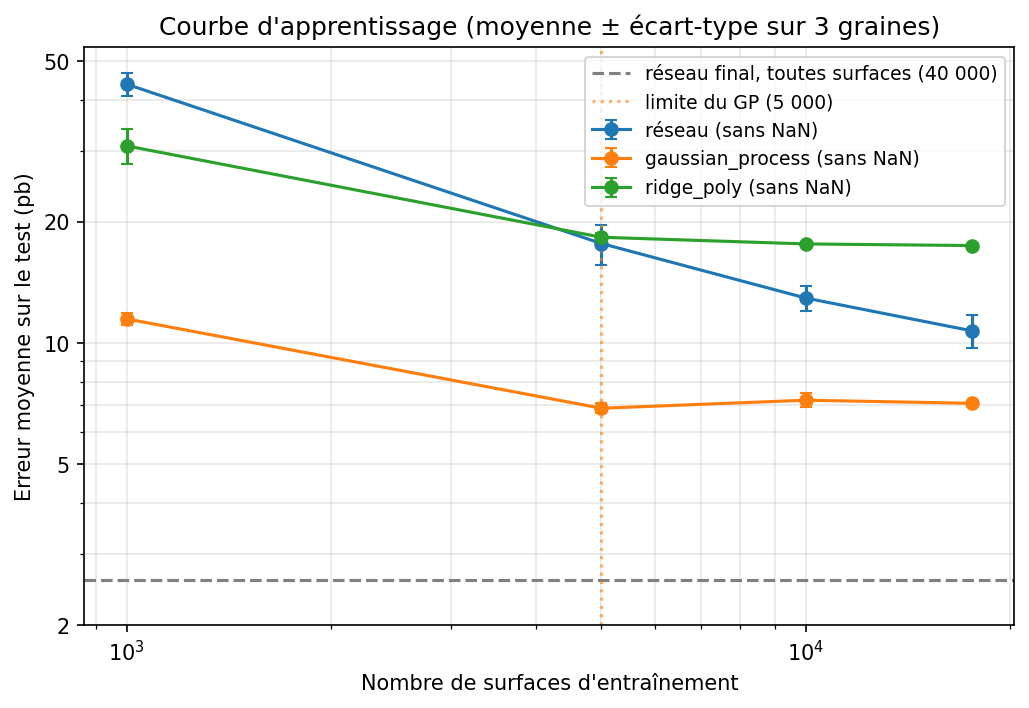
\includegraphics[width=0.75\textwidth]{etape3_courbe_apprentissage}
  \caption{Erreur moyenne sur le test selon le nombre de surfaces d'entraînement sans NaN (moyenne $\pm$
  écart-type sur 3 graines, échelles logarithmiques). Pointillés gris : réseau final entraîné sur les
  \num{40000} surfaces. Pointillés orange : limite de \num{5000} surfaces du GP.}
  \label{fig-ml-courbe}
\end{figure}

\begin{table}[H]
  \centering
  \caption{Erreur moyenne sur le test (pb, moyenne $\pm$ écart-type sur 3 graines) selon le nombre de surfaces
  d'entraînement.}
  \label{tab-ml-courbe}
  \small
  \begin{tabular}{rccc}
    \toprule
    Surfaces & Réseau & Processus gaussien & Ridge polynomiale \\
    \midrule
    \num{1000}  & $43{,}9 \pm 3{,}0$ & $11{,}5 \pm 0{,}4$ & $30{,}8 \pm 3{,}1$ \\
    \num{5000}  & $17{,}7 \pm 2{,}0$ & $6{,}89 \pm 0{,}19$ & $18{,}3 \pm 0{,}4$ \\
    \num{10000} & $12{,}9 \pm 1{,}0$ & $7{,}21 \pm 0{,}29$ & $17{,}6 \pm 0{,}1$ \\
    \num{17569} & $10{,}7 \pm 1{,}0$ & $7{,}09$ & $17{,}4$ \\
    \bottomrule
  \end{tabular}
\end{table}

Avec peu de données, le GP l'emporte nettement : \num{11.5}\pb\ avec \num{1000} surfaces, contre \num{43.9}\pb\
pour le réseau (\cref{fig-ml-courbe}, \cref{tab-ml-courbe}). La ridge plafonne autour de \num{17.5}\pb\ dès
\num{5000} surfaces : un polynôme de degré 4 ne peut pas faire mieux, quelle que soit la quantité de données. Le GP
plafonne à son tour à \num{5000} surfaces, à cause de sa limite de taille. Le réseau est le seul modèle dont
l'erreur baisse encore au bout de la courbe : \num{43.9}, puis \num{17.7}, \num{12.9} et \num{10.7}\pb. Sur les
\num{17569} surfaces, il ne rattrape pas le GP. Avec les \num{40000} surfaces, NaN compris, il descend à
\num{2.58}\pb.

\subsection{Bilan}
\label{sec-ml-bilan}

Sur un petit jeu de surfaces complètes, un processus gaussien est plus précis que notre réseau, pour un temps de
réponse qui passe encore le seuil. Le réseau prend l'avantage pour deux raisons. Son erreur continue de baisser
quand on ajoute des données, alors que le GP est limité par son coût et la ridge par sa forme. Et la perte masquée
lui permet d'apprendre sur toutes les surfaces, y compris les \SI{56}{\percent} qui ont un point manquant et qu'il
faut retirer pour les modèles classiques. Avec toutes les données, il fait \num{2.58}\pb\ sur le test, 2,7 fois
mieux que le GP, avec une erreur maximale de \num{93}\pb\ contre plus de \num{500}\pb\ pour tous les modèles
classiques, et il répond 5 à 6 fois plus vite.

Cette comparaison a ses limites. Les grilles d'hyperparamètres des modèles classiques sont petites, alors que le
réseau a été réglé en détail aux \cref{sec-architectures,sec-entrainement}. Nous n'avons pas essayé de compléter
les points manquants par imputation pour garder toutes les surfaces côté ML. Enfin, le coût du GP sur
\num{40000} surfaces est estimé à partir de sa complexité, pas mesuré.

% Étape 4 : calibration. Sources : notebooks/04_calibration.ipynb, results/calibration_*.csv, results/figures/etape4_calibration_spx.png, data/spx_surface.npz.

\section{Calibration et seuil de rentabilité}
\label{sec-calibration}

Dans cette dernière étape, nous utilisons le réseau retenu ($2 \times 128$ neurones, initialisation de He,
activation GELU, entraîné avec Adam) pour de vraies calibrations, et nous le comparons au pricer de référence par
transformée de Fourier (méthode COS).

\subsection{Protocole expérimental}

Le réseau et Fourier utilisent le même optimiseur, pour que seule la façon de calculer une surface change :
Levenberg-Marquardt, avec la fonction \texttt{least\_squares} de SciPy. Les bornes des cinq paramètres
$\Theta = (v_0, \theta, \kappa, \xi, \rho)$ sont imposées par un changement de variable sigmoïde, et les points
manquants (\texttt{NaN}) de la surface cible sont ignorés dans les résidus. Chaque calibration part des mêmes
$N_{\text{starts}} = 5$ points de départ, tirés par hypercube latin (graine $0$).

\subsection{Calibration sur surfaces simulées}

Nous comparons d'abord les deux méthodes sur $100$ surfaces du jeu de test (graine $42$), dont nous connaissons les
vrais paramètres $\Theta^*$. Le \cref{tab-calib-simulee} donne le taux de convergence, l'erreur d'ajustement sur les
volatilités implicites (en points de base, $1~\text{pb} = 10^{-4}$), l'erreur relative sur chaque paramètre
(rapportée à la largeur de sa plage) et le temps de calcul complet.

\begin{table}[htbp]
\centering
\caption{Performances comparées de la calibration sur $100$ surfaces du jeu de test ($5$ points de départ par surface).}
\label{tab-calib-simulee}
\small
\setlength{\tabcolsep}{4pt}
\begin{tabular}{lcccccc}
\toprule
 & \multicolumn{3}{c}{\textbf{Réseau de neurones}} & \multicolumn{3}{c}{\textbf{Fourier (COS Python)}} \\
\cmidrule(lr){2-4} \cmidrule(lr){5-7}
\textbf{Métrique} & \textbf{Moyenne} & \textbf{Médiane} & \textbf{Max} & \textbf{Moyenne} & \textbf{Médiane} & \textbf{Max} \\
\midrule
Taux de convergence & \multicolumn{3}{c}{$100\,\%$} & \multicolumn{3}{c}{$100\,\%$} \\
Erreur d'ajustement (pb) & $1{,}25$ & $1{,}12$ & $3{,}09$ & $2{,}23$ & $0{,}00$ & $67{,}60$ \\
Erreur maximale (pb) & $5{,}18$ & $4{,}59$ & $14{,}89$ & $10{,}28$ & $0{,}00$ & $212{,}80$ \\
Temps par calibration (s) & $0{,}0541$ & $0{,}0445$ & $0{,}3820$ & $34{,}8128$ & $25{,}3025$ & $173{,}5981$ \\
Nombre d'évaluations & $359{,}0$ & $330{,}0$ & $3097{,}0$ & $793{,}1$ & $611{,}5$ & $2654{,}0$ \\
\midrule
Erreur relative $v_0$ (\%) & $0{,}11\,\%$ & $0{,}08\,\%$ & $0{,}63\,\%$ & $0{,}25\,\%$ & $0{,}00\,\%$ & $4{,}19\,\%$ \\
Erreur relative $\theta$ (\%) & $0{,}08\,\%$ & $0{,}05\,\%$ & $1{,}35\,\%$ & $0{,}10\,\%$ & $0{,}00\,\%$ & $4{,}70\,\%$ \\
Erreur relative $\kappa$ (\%) & $0{,}33\,\%$ & $0{,}22\,\%$ & $1{,}90\,\%$ & $1{,}53\,\%$ & $0{,}00\,\%$ & $36{,}17\,\%$ \\
Erreur relative $\xi$ (\%) & $0{,}17\,\%$ & $0{,}15\,\%$ & $0{,}75\,\%$ & $0{,}56\,\%$ & $0{,}00\,\%$ & $9{,}86\,\%$ \\
Erreur relative $\rho$ (\%) & $0{,}36\,\%$ & $0{,}17\,\%$ & $4{,}67\,\%$ & $1{,}06\,\%$ & $0{,}00\,\%$ & $17{,}12\,\%$ \\
\bottomrule
\end{tabular}
\end{table}

Une calibration complète prend en moyenne $54{,}1~\text{ms}$ avec le réseau, contre $34{,}81~\text{s}$ avec le
pricer Fourier en Python : le réseau va $643{,}6$ fois plus vite. Le gain a deux origines. Le réseau évalue une
surface en NumPy pur en $0{,}176~\text{ms}$, normalisation par les scalers et mise en forme des tableaux comprises ;
la passe avant elle-même n'en prend que $0{,}028~\text{ms}$. Sa surface est aussi plus lisse, et l'optimiseur a
besoin de deux fois moins d'évaluations ($359$ contre $793$).

La précision ne se dégrade pas pour autant. L'erreur d'ajustement du réseau est de $1{,}12~\text{pb}$ en médiane
($1{,}25~\text{pb}$ en moyenne), bien en deçà des écarts observables sur les marchés d'options, et les cinq
paramètres sont retrouvés à moins de $0{,}22\,\%$ de la largeur de leur domaine en médiane.

Fourier atteint $0{,}00~\text{pb}$ en médiane, ce qui est attendu : les surfaces de test ont été générées par ce même
modèle. Il reste en revanche sensible à des minima locaux sur certaines configurations extrêmes, où son erreur
monte jusqu'à $67{,}60~\text{pb}$. Celle du réseau ne dépasse pas $3{,}09~\text{pb}$ sur tout le jeu de test.

\subsection{Calibration sur données de marché (SPX)}

Nous calibrons ensuite avec les deux méthodes les quatre surfaces réelles d'options sur l'indice S\&P 500 de
\texttt{spx\_surface.npz} ($3$, $4$, $5$ et $20$ novembre), restreintes à la zone de calibration de la
\cref{sec-spx} : $K/F \in [0{,}7\,;\,1{,}3]$ et $T \ge 0{,}3~\text{an}$, soit $46$ à $49$ points valides sur $88$
selon la date. Cette zone écarte les maturités très courtes, où le modèle de Heston ne parvient pas à reproduire le
\textit{skew} prononcé du marché.

\begin{table}[htbp]
\centering
\caption{Calibration comparée sur les quatre surfaces réelles SPX ($5$ points de départ par surface).}
\label{tab-calib-spx}
\resizebox{\textwidth}{!}{%
\begin{tabular}{llccccccccc}
\toprule
\textbf{Date} & \textbf{Méthode} & \textbf{Err. moy. (pb)} & \textbf{Err. max (pb)} & \textbf{Temps (s)} & \textbf{Éval.} & $v_0$ & $\theta$ & $\kappa$ & $\xi$ & $\rho$ \\
\midrule
2026-11-03 & Réseau & $28{,}57$ & $145{,}59$ & $0{,}173$ & $635$ & $0{,}0361$ & $0{,}0495$ & $3{,}8965$ & $1{,}5000$ & $-0{,}7187$ \\
 & Fourier & $29{,}20$ & $146{,}14$ & $33{,}831$ & $397$ & $0{,}0362$ & $0{,}0493$ & $3{,}8851$ & $1{,}5000$ & $-0{,}7195$ \\
\midrule
2026-11-04 & Réseau & $28{,}58$ & $124{,}18$ & $0{,}043$ & $358$ & $0{,}0230$ & $0{,}0486$ & $3{,}9827$ & $1{,}5000$ & $-0{,}7122$ \\
 & Fourier & $29{,}49$ & $125{,}18$ & $39{,}762$ & $438$ & $0{,}0231$ & $0{,}0485$ & $3{,}9944$ & $1{,}5000$ & $-0{,}7131$ \\
\midrule
2026-11-05 & Réseau & $28{,}51$ & $165{,}27$ & $0{,}132$ & $1094$ & $0{,}0526$ & $0{,}0507$ & $3{,}8410$ & $1{,}5000$ & $-0{,}7509$ \\
 & Fourier & $29{,}05$ & $165{,}70$ & $27{,}160$ & $427$ & $0{,}0530$ & $0{,}0505$ & $3{,}8145$ & $1{,}5000$ & $-0{,}7518$ \\
\midrule
2026-11-20 & Réseau & $29{,}22$ & $123{,}17$ & $0{,}034$ & $272$ & $0{,}0760$ & $0{,}0555$ & $3{,}9106$ & $1{,}5000$ & $-0{,}7597$ \\
 & Fourier & $29{,}85$ & $123{,}72$ & $35{,}644$ & $466$ & $0{,}0764$ & $0{,}0552$ & $3{,}8858$ & $1{,}5000$ & $-0{,}7614$ \\
\bottomrule
\end{tabular}%
}
\end{table}

Sur les quatre jours, le réseau donne les mêmes calibrations que Fourier (\cref{tab-calib-spx},
\cref{fig-calib-spx}). Les paramètres sont presque identiques d'une méthode à l'autre : l'écart est inférieur à
$0{,}0005$ sur $v_0$ et $\theta$, et à $0{,}0018$ sur $\rho$. L'erreur d'ajustement au marché est la même, entre
$28{,}5$ et $29{,}8~\text{pb}$ environ ; elle vient des limites du modèle de Heston à deux facteurs, pas du réseau.
Le temps moyen par journée passe en revanche de $34{,}10~\text{s}$ à $0{,}095~\text{s}$ : le réseau va environ
$360$ fois plus vite, et plus de $1000$ fois le 20 novembre.

\begin{figure}[htbp]
\centering
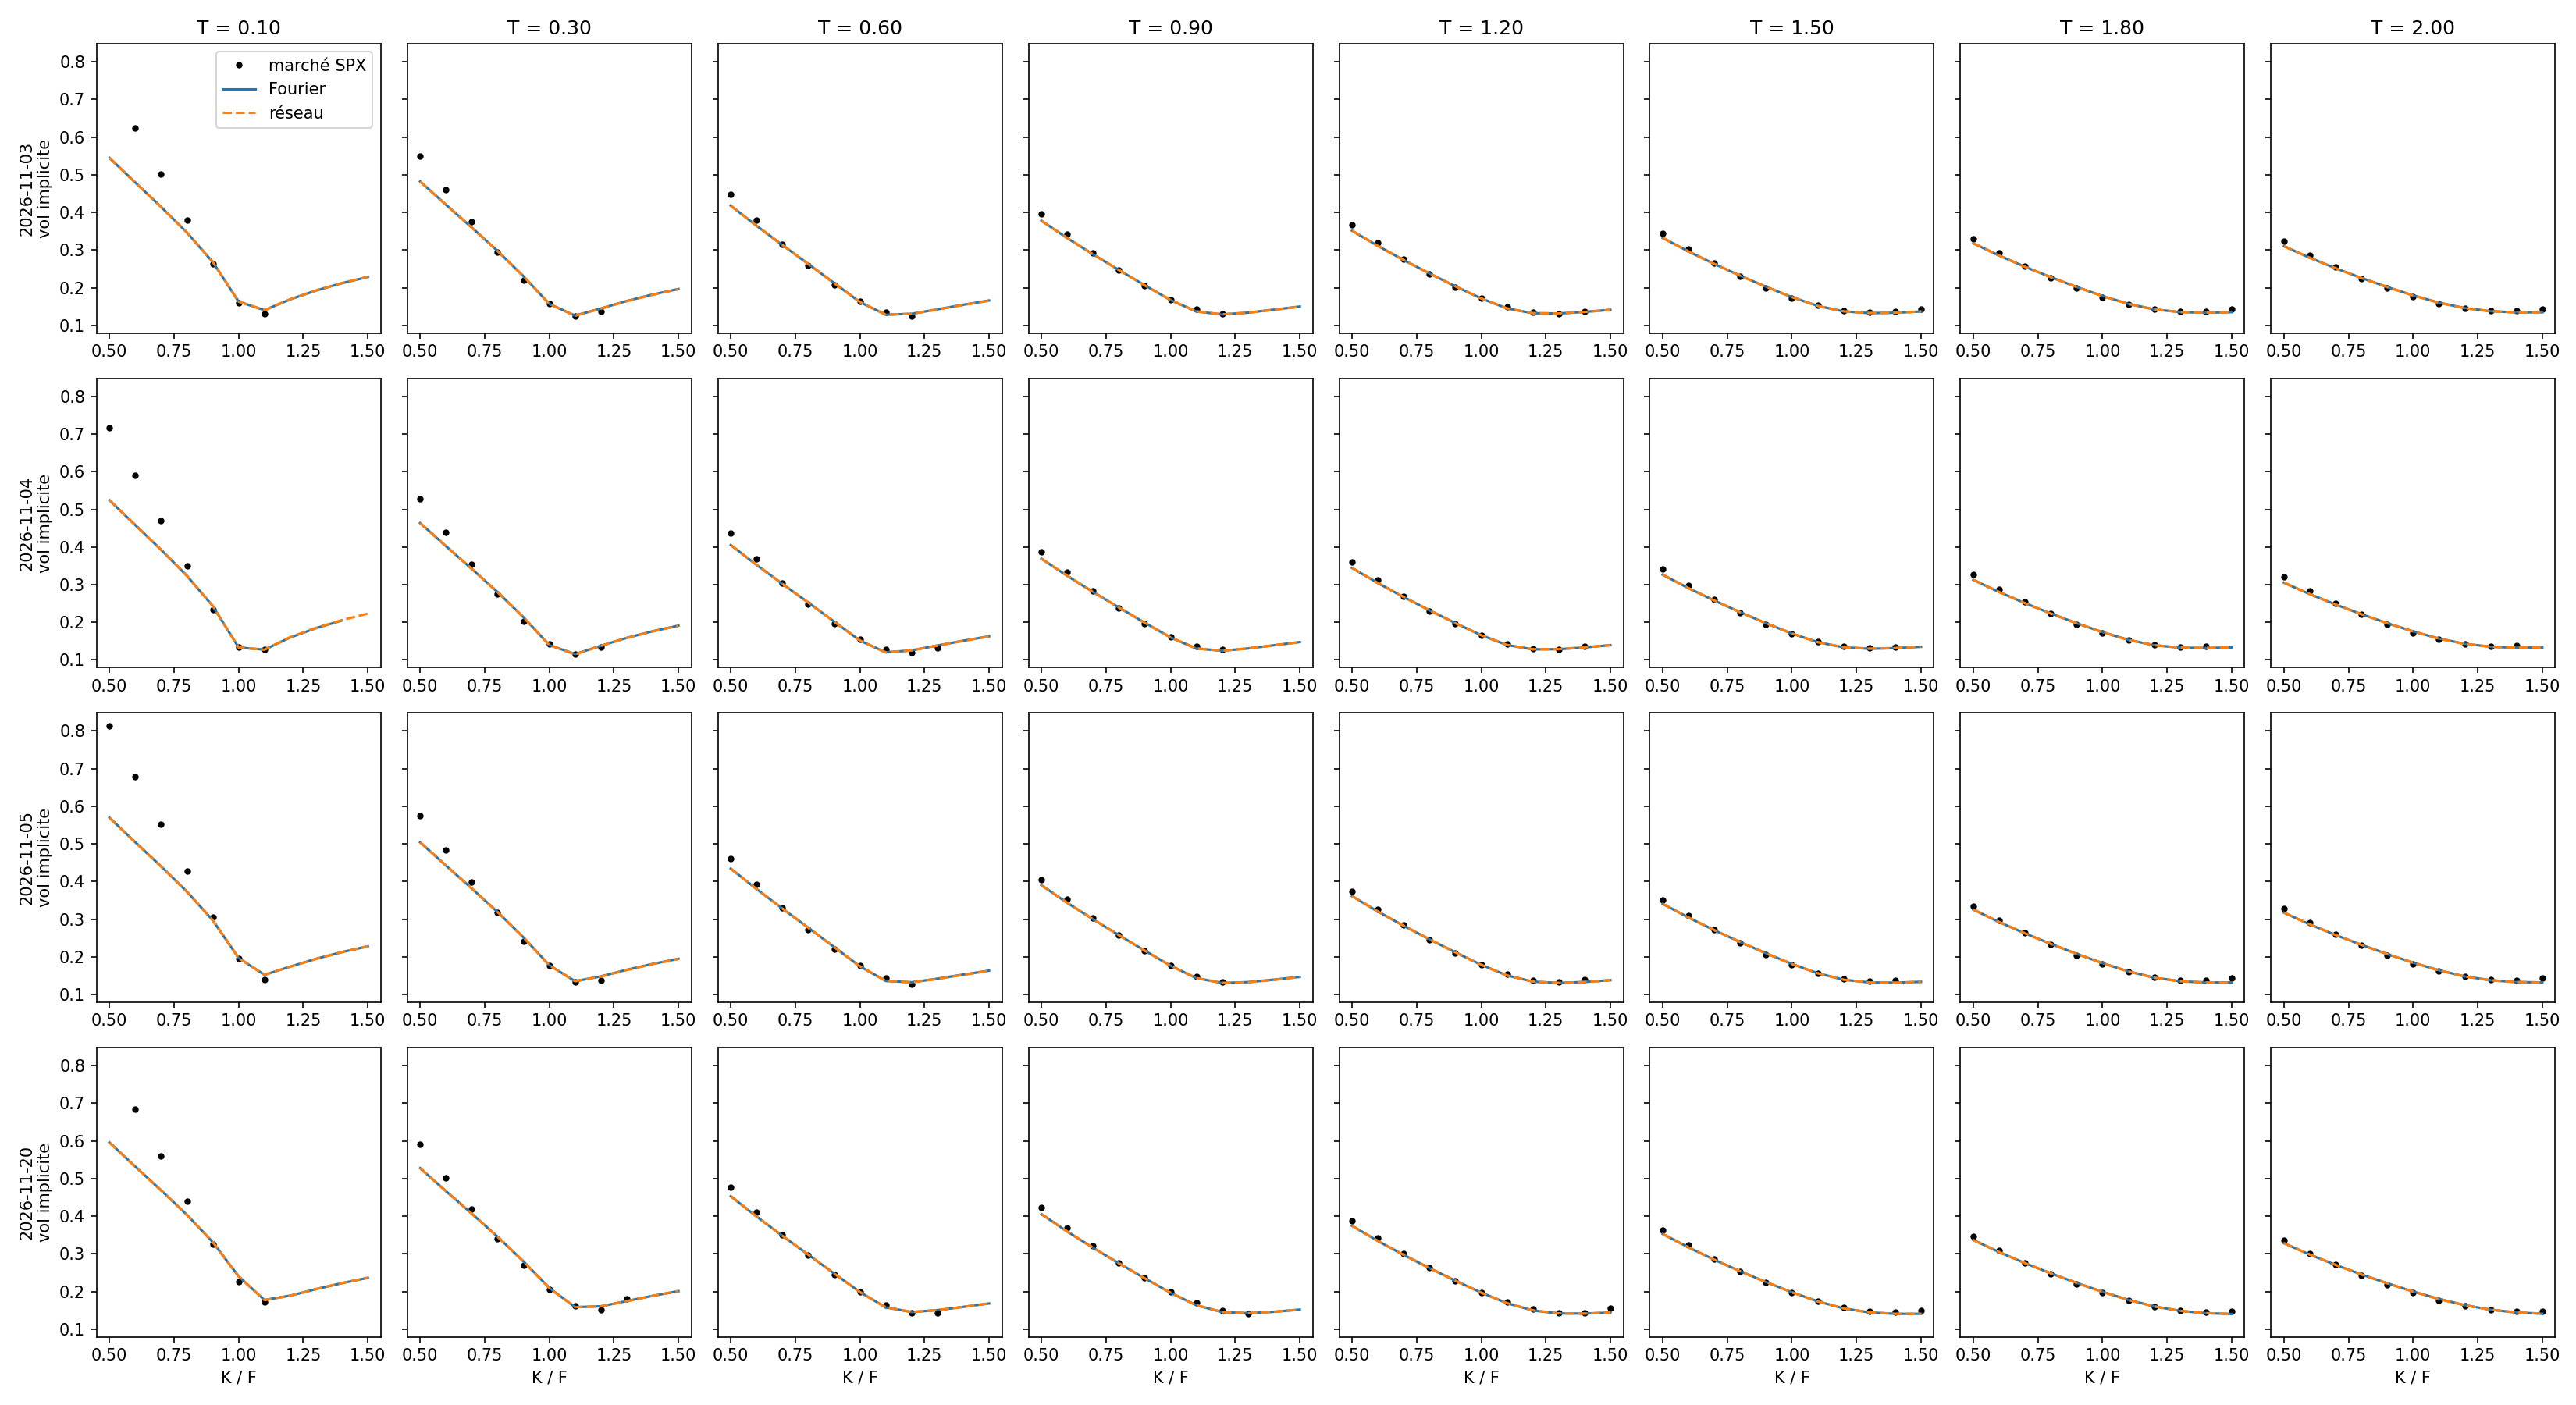
\includegraphics[width=\textwidth]{../results/figures/etape4_calibration_spx.png}
\caption{Superposition des volatilités implicites du marché SPX et des surfaces calibrées par Fourier et par le réseau de neurones sur les quatre dates étudiées.}
\label{fig-calib-spx}
\end{figure}

\subsection{Seuil de rentabilité}

Le réseau a un coût fixe, payé une seule fois : la génération des $50\,000$ surfaces d'apprentissage
($T_{\text{génération}} = 23{,}9~\text{s}$ en Julia) et l'entraînement du modèle final
($T_{\text{entraînement}} = 136{,}0~\text{s}$), soit $159{,}9~\text{s}$ au total. Le seuil de rentabilité $n^*$ est
le nombre de calibrations à partir duquel ce coût est amorti :
\begin{equation}
n^* = \left\lceil \frac{T_{\text{génération}} + T_{\text{entraînement}}}{t_{\text{calib, Fourier}} - t_{\text{calib, réseau}}} \right\rceil
\end{equation}

Avec les temps moyens mesurés sur le jeu de test ($t_{\text{calib, Fourier}} = 34{,}813~\text{s}$ et
$t_{\text{calib, réseau}} = 0{,}0541~\text{s}$), chaque calibration fait gagner $34{,}76~\text{s}$, et le seuil vaut :
\[
n^* = \left\lceil \frac{23{,}9 + 136{,}0}{34{,}813 - 0{,}0541} \right\rceil = 5 \text{ calibrations} \quad (\text{valeur exacte } 4{,}60).
\]
Si l'on compare plutôt au pricer de référence en Julia ($2{,}29~\text{ms}$ par surface sur un cœur, soit environ
$1{,}82~\text{s}$ pour $793$ évaluations), le gain tombe à $1{,}76~\text{s}$ par calibration, et le réseau est
rentable à partir de $n^* = 91$ calibrations. En production, ce volume est atteint dès la première journée de
cotation.

% Conclusion.

\section{Conclusion}
\label{sec-conclusion}

Nous avons appliqué au modèle de Heston la méthode de \citet{horvath2021} : apprendre une fois pour toutes la
fonction qui associe aux cinq paramètres la surface de volatilité, puis calibrer avec le réseau à la place du
pricer de Fourier. Elle fonctionne.

\paragraph{Le réseau.} Un petit réseau suffit. Le $2\times128$ est le plus précis des réseaux assez rapides : les
plus grands sont plus précis mais trop lents, et ajouter des couches n'aide pas. Le choix de l'entraînement compte
autant que la taille : avec Adam, l'initialisation de He et l'activation GELU, l'erreur passe de \num{5.09} à
\num{2.67}\pb\ sur le test, pour le même temps de réponse, plus de 70 fois plus court que celui de
Fourier en Julia. Ces choix ne s'additionnent pas : le meilleur réglage d'un hyperparamètre dépend des autres.

\paragraph{Réseau ou apprentissage classique.} Sur un petit jeu de surfaces complètes, un processus gaussien est
plus précis que le réseau. Le réseau l'emporte pour deux raisons : son erreur baisse encore quand on ajoute des
données, et la perte masquée lui permet d'apprendre sur toutes les surfaces, y compris celles qui ont un point
manquant. Avec toutes les données, il est 2,7 fois plus précis que le GP et son erreur maximale est cinq fois plus
petite.

\paragraph{La calibration.} Sur 100 surfaces simulées, le réseau retrouve les paramètres à moins de
\SI{0.22}{\percent} de leur plage en médiane, avec une erreur d'ajustement de \num{1.12}\pb, et calibre environ
640 fois plus vite que Fourier en Python. Sur les quatre jours de SPX, il donne les mêmes paramètres et la même
erreur que Fourier (environ \num{29}\pb), en un dixième de seconde au lieu d'une trentaine de secondes. Le coût de la
génération des données et de l'entraînement est amorti dès 5 calibrations face à Fourier en Python, et vers
\num{90} face à Julia : bien moins que ce qu'une banque calibre en une journée.

\paragraph{Limites.} L'erreur sur le SPX vient du modèle, pas du réseau : Heston ne reproduit pas le skew à un mois,
$\xi$ atteint sa borne, et nous avons dû calibrer sur une zone réduite de la surface. Nos données de marché couvrent
quatre jours de novembre 2026, dans un seul régime de volatilité. Enfin, le réseau ne connaît que le domaine sur
lequel il a appris : une surface qui en sort devrait être recalibrée avec Fourier, ou le réseau réentraîné.

\paragraph{Pistes.} Le gain serait bien plus grand pour un modèle sans pricer rapide. Pour les modèles à volatilité
rugueuse \citep{gatheral2018}, qui reproduisent mieux le skew court du SPX, chaque surface demande une simulation de
Monte-Carlo : c'est là que la méthode prend tout son intérêt, comme le montrent \citet{horvath2021}. Une base de
données historique permettrait aussi de tester la calibration sur plusieurs régimes de marché, calmes comme en
crise.


\bibliographystyle{plainnat}
\bibliography{references}

\end{document}
